\documentclass[11pt,a4paper]{ctexart}

% ============================ 宏包 ============================
\usepackage{amsmath,amssymb,amsthm,mathtools}
\usepackage{geometry}
\geometry{left=2.3cm,right=2.3cm,top=2.5cm,bottom=2.4cm}
\usepackage{graphicx}
\usepackage{float}
\usepackage{caption}
\usepackage{xcolor}
\usepackage{enumitem}
\usepackage{booktabs}
\usepackage{array}
\usepackage{tikz}
\usetikzlibrary{arrows.meta,positioning,decorations.pathreplacing,calc,patterns}
\usepackage{fancyhdr}
\usepackage{tcolorbox}
\tcbuselibrary{skins,breakable}
\usepackage{titlesec}
\usepackage{hyperref}
\hypersetup{colorlinks=true,linkcolor=teal!60!black,
            urlcolor=teal!60!black,citecolor=teal!60!black}

% ============================ 字体与格式 ============================
\setCJKmainfont{SimSun}[BoldFont=SimHei,ItalicFont=KaiTi]
\setCJKsansfont{Microsoft YaHei}
\setCJKfamilyfont{kai}{KaiTi}
\providecommand{\kaishu}{}
\renewcommand{\kaishu}{\CJKfamily{kai}}

\definecolor{mainc}{RGB}{31,78,121}
\definecolor{upc}{RGB}{192,57,43}
\definecolor{downc}{RGB}{30,132,73}
\definecolor{orangec}{RGB}{230,126,34}
\definecolor{purplec}{RGB}{108,52,131}
\definecolor{lightbg}{RGB}{246,248,251}

\captionsetup[figure]{font=small,labelfont={bf,color=mainc},
                      labelsep=quad,textfont=small}
\captionsetup[table]{font=small,labelfont={bf}}

\titleformat{\section}{\Large\bfseries\color{mainc}}{\thesection}{0.8em}{}
\titleformat{\subsection}{\large\bfseries\color{mainc}}{\thesubsection}{0.7em}{}
\titleformat{\subsubsection}{\normalsize\bfseries}{\thesubsubsection}{0.6em}{}
\titlespacing*{\section}{0pt}{1.6em}{0.8em}

\setlist[itemize]{leftmargin=1.6em,itemsep=2pt,topsep=4pt}
\setlist[enumerate]{leftmargin=1.9em,itemsep=2pt,topsep=4pt}

\linespread{1.28}

% 定理环境
\theoremstyle{definition}
\newtheorem{theorem}{定理}[section]
\newtheorem{lemma}[theorem]{引理}
\newtheorem{corollary}[theorem]{推论}
\newtheorem{example}[theorem]{例}
\newtheorem{proposition}[theorem]{命题}

\theoremstyle{remark}
\newtheorem*{remark}{注}
\newtheorem*{proofidea}{思路}

\renewcommand{\proofname}{\bfseries 证明}
\renewcommand\qedsymbol{$\blacksquare$}

% 常用记号
\newcommand{\R}{\mathbb{R}}
\newcommand{\N}{\mathbb{N}}
\newcommand{\Q}{\mathbb{Q}}
\newcommand{\eps}{\varepsilon}
\newcommand{\dd}{\,\mathrm{d}}
\DeclareMathOperator*{\esssup}{ess\,sup}
\newcommand{\abs}[1]{\left\lvert #1 \right\rvert}
\newcommand{\norm}[1]{\left\lVert #1 \right\rVert}

% 自定义盒子
\newtcolorbox{keybox}[1][]{
  colback=lightbg, colframe=mainc, boxrule=0.7pt, arc=2pt,
  left=7pt,right=7pt,top=5pt,bottom=5pt,
  fonttitle=\bfseries\color{white}, coltitle=white,
  colbacktitle=mainc, title={#1},
  breakable, enhanced
}

\newtcolorbox{warnbox}[1][]{
  colback=orangec!6, colframe=orangec!85!black, boxrule=0.7pt, arc=2pt,
  left=7pt,right=7pt,top=5pt,bottom=5pt,
  fonttitle=\bfseries\color{white}, coltitle=white,
  colbacktitle=orangec!85!black, title={#1},
  breakable, enhanced
}

\newtcolorbox{tipbox}[1][]{
  colback=downc!6, colframe=downc!80!black, boxrule=0.7pt, arc=2pt,
  left=7pt,right=7pt,top=5pt,bottom=5pt,
  fonttitle=\bfseries\color{white}, coltitle=white,
  colbacktitle=downc!80!black, title={#1},
  breakable, enhanced
}

% 页眉页脚
\pagestyle{fancy}
\fancyhf{}
\fancyhead[L]{\small\color{mainc} 数学分析专题笔记}
\fancyhead[R]{\small\color{mainc} 不等式与放缩法}
\fancyfoot[C]{\small\thepage}
\renewcommand{\headrulewidth}{0.4pt}
\renewcommand{\headrule}{\hbox to\headwidth{\color{mainc}\leaders\hrule height \headrulewidth\hfill}}

% 图文并排用
\newcommand{\figph}[2][0.85]{%
  \begin{figure}[H]\centering
  \includegraphics[width=#1\textwidth]{figures/#2}
  \end{figure}}

\begin{document}

% ============================ 封面 ============================
\begin{titlepage}
\centering
\vspace*{2.2cm}

{\color{mainc}\rule{\linewidth}{1.6pt}}\\[0.9cm]

{\Huge\bfseries 数学分析中的\par}
\vspace{0.35cm}
{\Huge\bfseries 常用不等式与放缩法\par}
\vspace{0.35cm}
{\LARGE\bfseries 完整图像 · 严格证明 · 典型例题\par}

\vspace{0.6cm}
{\color{mainc}\rule{\linewidth}{1.6pt}}

\vspace{2.6cm}

{\large\kaishu
\begin{tabular}{rl}
\textbf{主题} & 均值不等式 · 柯西—施瓦茨 · 伯努利 · 对数与指数\\[3pt]
              & 三角不等式 · 积分不等式 · Young · 排序与 Chebyshev\\[3pt]
\textbf{核心方法} & 放缩法（两边夹、逐项放缩、裂项放缩、\\[3pt]
              & 积分放缩、单调性放缩、切线放缩）\\[3pt]
\textbf{适用} & 极限证明 · 级数敛散性 · 估值与比较\\[3pt]
\end{tabular}}

\vfill

{\large 共收录 \textbf{12} 幅手绘级矢量插图、\textbf{20} 条定理与引理}

\vspace{1.2cm}
{\color{mainc}\rule{0.45\linewidth}{0.8pt}}
\end{titlepage}

% ============================ 目录 ============================
\tableofcontents
\newpage

% ============================ 第 0 章 ============================
\section{引言：为什么“放缩”是数学分析的灵魂}

在数学分析中，我们极少能直接算出待求的量。更多的时候，我们只能判断它“大概有多大”，
并希望这种判断足够精确，以至于能夹出确定的结果。\textbf{放缩法}
（bounding / estimation）正是把“未知量”换成“已知量的上下界”的技术。

\subsection{放缩法的基本逻辑}

设待考察的量为 $X$。若能找到两个\emph{可以处理的}量 $L$ 与 $U$，使得
\begin{equation}\label{eq:squeeze-basic}
  L\ \le\ X\ \le\ U,
\end{equation}
并且 $L$ 与 $U$ 在某种极限意义下相等（$L\to A$ 且 $U\to A$），则由夹逼原理 $X\to A$。
图~\ref{fig:sandwich} 给出了这一结构的几何图像：放缩的成败，本质上取决于
\textbf{上下界之差是否趋于零}。

\begin{figure}[H]
  \centering
  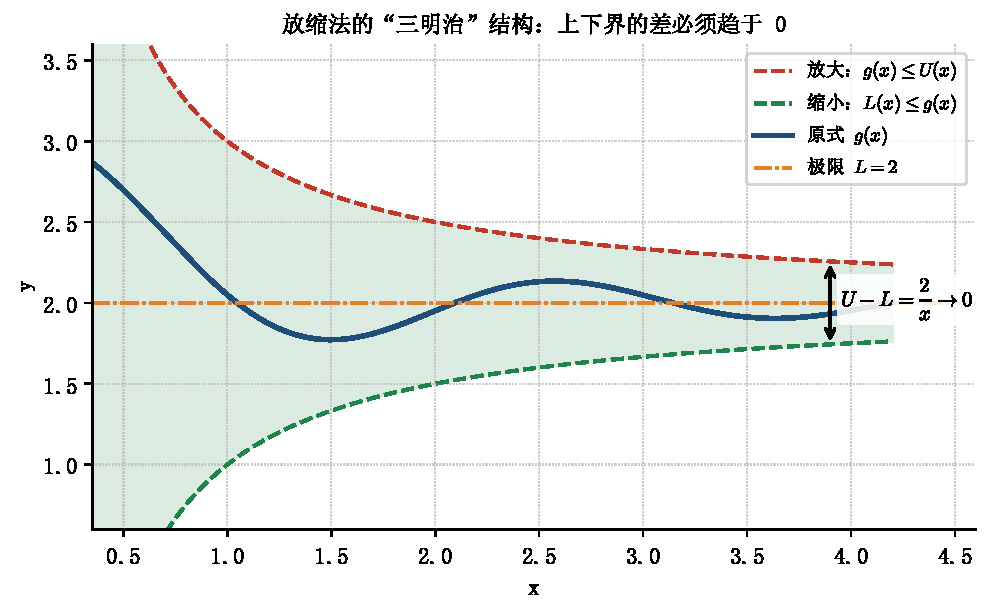
\includegraphics[width=0.86\textwidth]{figures/fig8_sandwich.pdf}
  \caption{放缩法的“三明治”结构。上下界曲线 $L(x)\le g(x)\le U(x)$ 之间的带宽
           $\frac2x\to0$ 时，$g(x)$ 被迫收敛到同一极限 $L=2$。}
  \label{fig:sandwich}
\end{figure}

% ------------------------------------------------------------------
\subsection{放缩的“松紧”权衡}

放缩法有一个内在矛盾，值得一开始就说清楚：

\begin{keybox}[放缩法的两难]
\begin{itemize}
  \item \textbf{放得太松}：$U$ 与 $L$ 的极限不相等，夹逼失效，只能得到“有界”这种弱结论。
  \item \textbf{放得太紧}：每项都保留原样，等于什么也没做，仍然算不出来。
  \item \textbf{合适的放缩}：保留\emph{主要部分}，只丢弃\emph{可忽略的尾项}。
        典型做法是“保留前有限项，尾巴统一放缩”。
\end{itemize}
\end{keybox}

一个最朴素的例子能说明这一点。对 $0<a_1\le a_2\le\cdots\le a_n$，若令
$S=\sum_{k=1}^n a_k$，则
\[
  n\,a_1\ \le\ S\ \le\ n\,a_n .
\]
这个放缩永远成立，但它给出的界与 $n$ 同阶、且上下界比值是 $a_n/a_1$，
对求 $S$ 的精确渐近毫无用处。反之，如果已知 $a_k\to0$，则
$S=o(n)$ 的结论可以由
$S\le \max_{k\le \sqrt n} a_k\cdot \sqrt n + \frac{n}{\sqrt n}\cdot\max a_k$
这类\emph{分段放缩}得到，这就是“保留主要部分”的思想。

% ------------------------------------------------------------------
\subsection{本文的组织}

第一章列举\textbf{常用不等式}：每一条都给出\emph{图像}（用来说明它“为什么显然”）、
\emph{严格证明}（用来说明它“为什么正确”）、\emph{取等条件}
（用来说明它“什么时候最有用”）。第二章系统总结\textbf{放缩方法}：
按“逐项放缩—裂项—积分—单调性—切线”五种范式组织。
第三章给出一个\textbf{完整例题}，把两章内容串起来。

\bigskip
\begin{keybox}[符号约定]
全文中 $\N=\{1,2,3,\dots\}$；$a\wedge b=\min\{a,b\}$，$a\vee b=\max\{a,b\}$；
$f\lesssim g$ 表示存在常数 $C>0$ 使 $f\le Cg$（Cassini 记号）；
$f\sim g$ 表示 $f/g\to1$。
\end{keybox}

\newpage

% ============================ 第 1 章 ============================
\section{常用不等式：图像、证明与取等条件}

% ------------------------------------------------------------------
\subsection{均值不等式链}

\begin{theorem}[四均值不等式]\label{thm:means}
设 $a,b>0$，记
\[
  A=\frac{a+b}{2},\qquad G=\sqrt{ab},\qquad
  H=\frac{2ab}{a+b},\qquad \text{且 } \min\{a,b\}\le A,G,H\le \max\{a,b\},
\]
则有
\begin{equation}\label{eq:mean-chain}
  \frac{2ab}{a+b}\ \le\ \sqrt{ab}\ \le\ \frac{a+b}{2}
  \qquad\Longleftrightarrow\qquad H\le G\le A,
\end{equation}
且三者相等当且仅当 $a=b$。
\end{theorem}

\begin{figure}[H]
  \centering
  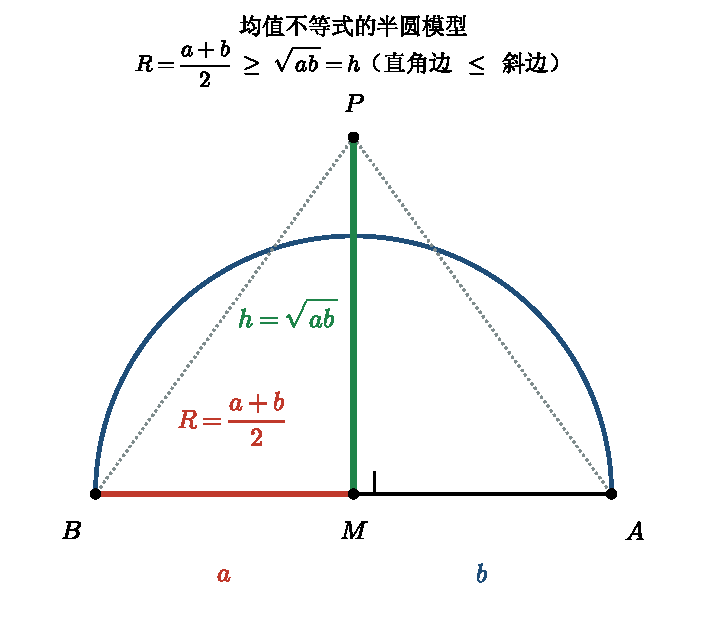
\includegraphics[width=0.80\textwidth]{figures/fig1_amgm.pdf}
  \caption{均值不等式的半圆模型：直径 $AB=a+b$ 被 $M$ 分成 $a,b$ 两段，
           半径 $MB=(a+b)/2$ 为算术平均，垂线 $MP=\sqrt{ab}$ 为几何平均。
           在直角三角形 $MPB$ 中直角边 $MP$ 小于斜边 $MB$，故 $\sqrt{ab}\le\frac{a+b}{2}$。}
  \label{fig:amgm}
\end{figure}

\begin{proof}
\textbf{第 1 步（代数）}：由 $(\sqrt a-\sqrt b)^2\ge0$ 展开得
\[
  a+b-2\sqrt{ab}\ \ge\ 0
  \quad\Longrightarrow\quad
  \sqrt{ab}\ \le\ \frac{a+b}{2},
\]
等号成立当且仅当 $\sqrt a=\sqrt b$，即 $a=b$。

\textbf{第 2 步（调和—几何）}：在已证结论中把 $a,b$ 换成 $1/a,\,1/b$（仍为正），得
\[
  \sqrt{\frac{1}{a}\cdot\frac{1}{b}}\ \le\ \frac{\frac1a+\frac1b}{2}
  \quad\Longrightarrow\quad
  \frac{2ab}{a+b}\ \le\ \sqrt{ab}.
\]
等号同样当且仅当 $a=b$。
\end{proof}

\begin{remark}[几何证明的要点]
图~\ref{fig:amgm} 中 $P$ 在半圆上，所以 $\angle APB=90^\circ$（半圆上的圆周角）。
在直角三角形 $APB$ 中作斜边上的高 $PM$，由射影定理
\[
  PM^2=AM\cdot MB=a\cdot b\quad\Longrightarrow\quad PM=\sqrt{ab}.
\]
而 $MB$ 是半径 $\frac{a+b}{2}$。直角三角形中直角边 $PM$ 短于斜边 $MB$，于是 $\sqrt{ab}\le\frac{a+b}{2}$，
当且仅当 $P$ 与 $M$ 重合（即 $a=b$）时取等。这个证明的美妙之处在于：
\emph{不等式的全部内容都在“直角边不长于斜边”这一句里}。
\end{remark}

\begin{figure}[H]
  \centering
  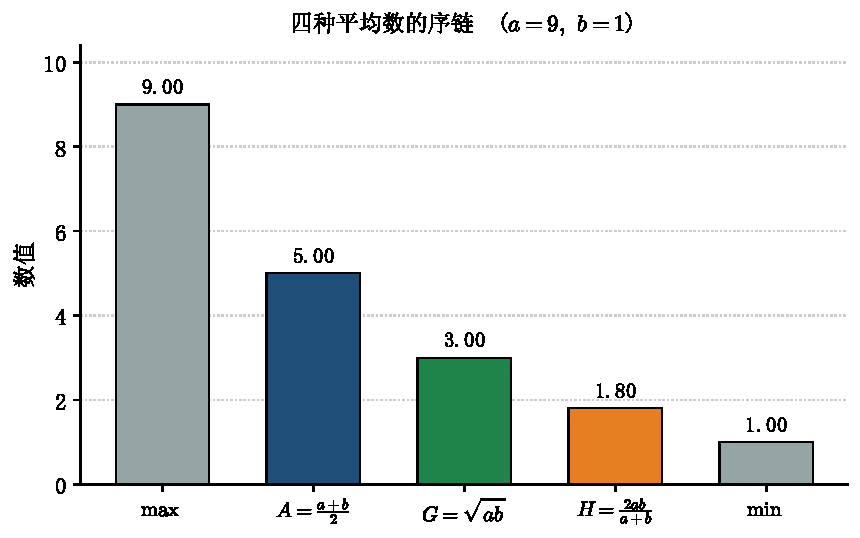
\includegraphics[width=0.72\textwidth]{figures/fig2_mean_chain.pdf}
  \caption{四种平均数的序链（取 $a=9,\ b=1$）：$1\le H=1.8\le G=3\le A=5\le 9$。
           当 $a,b$ 差距越大，四个量之间的“缝隙”越宽；当 $a\to b$ 时柱高趋于重合。}
  \label{fig:meanchain}
\end{figure}

\begin{corollary}[$n$ 元算术—几何平均不等式]\label{cor:amgm-n}
设 $a_1,\dots,a_n>0$，则
\begin{equation}\label{eq:amgm-n}
  \sqrt[n]{a_1a_2\cdots a_n}\ \le\ \frac{a_1+a_2+\cdots+a_n}{n},
\end{equation}
等号当且仅当 $a_1=\cdots=a_n$。
\end{corollary}

\begin{proof}[证明（向前—向后归纳法）]
记 $A_n=\frac1n\sum_{k=1}^n a_k$，$G_n=(a_1\cdots a_n)^{1/n}$。

\emph{第 1 步（$n=2$ 已证）}：即定理~\ref{thm:means}。

\emph{第 2 步（$n\Rightarrow 2n$）}：
\[
  \frac{1}{2n}\sum_{k=1}^{2n}a_k
  =\frac{1}{2}\Big(\underbrace{\frac{1}{n}\sum_{k=1}^{n}a_k}_{\ge G_n}
              +\underbrace{\frac{1}{n}\sum_{k=n+1}^{2n}a_k}_{\ge G'_n=(a_{n+1}\cdots a_{2n})^{1/n}}\Big)
  \ \ge\ \frac{G_n+G'_n}{2}
  \ \ge\ \sqrt{G_nG'_n}=G_{2n},
\]
两次用 $n=2$ 的结论。

\emph{第 3 步（$n\Rightarrow n-1$，即反向归纳）}：
给定 $a_1,\dots,a_{n-1}>0$，令
$a_n:=\frac{1}{n-1}\sum_{k=1}^{n-1}a_k=A_{n-1}$。对 $n$ 个数用 \eqref{eq:amgm-n}：
\[
  \Big(a_1\cdots a_{n-1}\cdot A_{n-1}\Big)^{1/n}
  \ \le\ \frac{1}{n}\Big(\sum_{k=1}^{n-1}a_k+A_{n-1}\Big)
  =\frac{(n-1)A_{n-1}+A_{n-1}}{n}=A_{n-1}.
\]
两边取 $n$ 次幂：$a_1\cdots a_{n-1}\cdot A_{n-1}\le A_{n-1}^{\,n}$，
即 $a_1\cdots a_{n-1}\le A_{n-1}^{\,n-1}$，开 $n-1$ 次方得
$G_{n-1}=\big(a_1\cdots a_{n-1}\big)^{\frac{1}{n-1}}\le A_{n-1}$。

于是由 $2$ 出发可到 $4,8,16,\dots$；再由反向归纳可向下覆盖全部正整数 $n$。
等号条件由每次取等的条件逐层回溯得到：$a_1=\cdots=a_n$。
\end{proof}

% ------------------------------------------------------------------
\subsection{柯西—施瓦茨不等式}

\begin{theorem}[Cauchy–Schwarz]\label{thm:cs}
设 $a_1,\dots,a_n,b_1,\dots,b_n\in\R$，则
\begin{equation}\label{eq:cs}
  \Big(\sum_{k=1}^{n}a_kb_k\Big)^{2}
  \ \le\ \Big(\sum_{k=1}^{n}a_k^{2}\Big)\Big(\sum_{k=1}^{n}b_k^{2}\Big),
\end{equation}
等号当且仅当 $(a_1,\dots,a_n)$ 与 $(b_1,\dots,b_n)$ 线性相关（成比例）。
\end{theorem}

\begin{figure}[H]
  \centering
  \begin{tikzpicture}[scale=1.0,>=Stealth]
    \coordinate (O) at (0,0);
    \coordinate (A) at (4.2,0.6);   % a 向量
    \coordinate (B) at (1.4,2.6);   % b 向量
    % 平行四边形
    \fill[downc!18] (O) -- (A) -- ($(A)+(B)$) -- (B) -- cycle;
    % 向量
    \draw[->,ultra thick,mainc] (O) -- (A) node[below right,mainc] {$\mathbf a$};
    \draw[->,ultra thick,upc]   (O) -- (B) node[above left,upc] {$\mathbf b$};
    % 投影
    \coordinate (P) at ($(O)!(B)!(A)$);
    \draw[dashed,gray] (B) -- (P);
    \draw[->,thick,orangec] (O) -- (P) node[below=1pt,orangec] {\small $b_{\parallel}$};
    % 矩形
    \draw[thick,gray,dashed] (A) -- ($(A)+(B)$) -- (B);
    % 直角标记
    \draw[gray] ($(P)+(-0.13,0.13)$) -- ($(P)+(0.13,0.13)$) -- ($(A)+(0.13,0.13)-(0.55,0)$);
    % 公式
    \node[anchor=west,align=left] at (6.4,2.0)
      {\small$\mathbf a\cdot\mathbf b=\norm{\mathbf a}\,\norm{\mathbf b}\cos\theta$};
    \node[anchor=west,align=left] at (6.4,1.05)
      {\small$\abs{\cos\theta}\le 1\ \Longrightarrow\ \abs{\mathbf a\cdot\mathbf b}\le\norm{\mathbf a}\norm{\mathbf b}$};
    \node[anchor=west,align=left] at (6.4,0.1)
      {\small 等号 $\iff\theta=0$ 或 $\pi$ $\iff$ 两向量共线};
    \draw[->,mainc] (4.0,0.0) .. controls (5.2,0.6) .. (6.2,1.0);
  \end{tikzpicture}
  \caption{柯西—施瓦茨不等式的几何本质：$\mathbf a\cdot\mathbf b$ 是“投影长度 $\norm{\mathbf a}\cos\theta$”
           与 $\norm{\mathbf b}$ 的乘积，其绝对值不超过两向量长度之积。}
  \label{fig:cs}
\end{figure}

\begin{proof}[证明一（判别式法）]
对任意实数 $t$（或复数 $t$ 取模），考虑非负二次型
\[
  q(t)=\sum_{k=1}^{n}(a_k t-b_k)^{2}\ \ge\ 0.
\]
展开：
\[
  q(t)=\Big(\sum a_k^{2}\Big)t^{2}-2\Big(\sum a_kb_k\Big)t+\Big(\sum b_k^{2}\Big)\ \ge\ 0
  \qquad\forall t\in\R.
\]
记 $A=\sum a_k^2$，$C=\sum a_kb_k$，$B=\sum b_k^2$。
若 $A=0$，则所有 $a_k=0$，\eqref{eq:cs} 两边均为 $0$，显然成立。
若 $A>0$，则开口向上的抛物线恒非负，判别式必 $\le 0$：
\[
  \Delta=4C^{2}-4AB\ \le\ 0\quad\Longrightarrow\quad C^{2}\le AB,
\]
此即 \eqref{eq:cs}。

等号成立当且仅当存在 $t_0$ 使 $q(t_0)=0$，即所有 $a_kt_0-b_k=0$，也就是
$b_k=t_0a_k$ 对所有 $k$ 成立。
\end{proof}

\begin{proof}[证明二（内积法，可直接推广到 $L^2$）]
设 $\mathbf b\neq\mathbf 0$，令 $\mathbf p=\frac{\langle\mathbf a,\mathbf b\rangle}{\norm{\mathbf b}^2}\,\mathbf b$
为 $\mathbf a$ 在 $\mathbf b$ 上的投影，则 $\mathbf a-\mathbf p\perp\mathbf b$，于是
\[
  \norm{\mathbf a}^{2}
  =\norm{\mathbf p}^{2}+\norm{\mathbf a-\mathbf p}^{2}
  \ \ge\ \norm{\mathbf p}^{2}
  =\frac{\langle\mathbf a,\mathbf b\rangle^{2}}{\norm{\mathbf b}^{2}}.
\]
两边乘 $\norm{\mathbf b}^2$ 即得。这正是图~\ref{fig:cs} 的勾股分解。
\end{proof}

\begin{keybox}[柯西不等式的四种常用变形]
\begin{enumerate}[label=(\arabic*)]
  \item \textbf{Titu 引理（分式型）}：$a_k>0,\ b_k>0$ 时
        \[
          \sum_{k=1}^{n}\frac{b_k^{2}}{a_k}\ \ge\ \frac{\Big(\sum b_k\Big)^{2}}{\sum a_k}.
        \]
  \item \textbf{乘积型}：$\Big(\sum a_kb_k\Big)^2\le\sum a_k^2\cdot\sum b_k^2$
        在 $b_k=1$ 时退化为 $n\sum a_k^2\ge\big(\sum a_k\big)^2$。
  \item \textbf{积分型}：$f,g\in\mathcal R[a,b]$ 时
        $\Big(\int_a^b fg\Big)^{2}\le\int_a^b f^{2}\cdot\int_a^b g^{2}$。
  \item \textbf{函数型}：$\big(\mathbb E[XY]\big)^{2}\le\mathbb E[X^{2}]\,\mathbb E[Y^{2}]$
        （概率形式，即 $\abs{\rho}\le 1$）。
\end{enumerate}
\end{keybox}

% ------------------------------------------------------------------
\subsection{伯努利不等式}

\begin{theorem}[Bernoulli]\label{thm:bernoulli}
设 $x>-1$，$n\in\N$，则
\begin{equation}\label{eq:bernoulli}
  (1+x)^{n}\ \ge\ 1+nx .
\end{equation}
若 $n\ge 2$ 且 $x\neq 0$，则不等号严格。更一般地，对实数 $\alpha\ge1$ 或 $\alpha\le0$，
\((1+x)^{\alpha}\ge 1+\alpha x\)；对 $0<\alpha<1$ 不等号反向。
\end{theorem}

\begin{figure}[H]
  \centering
  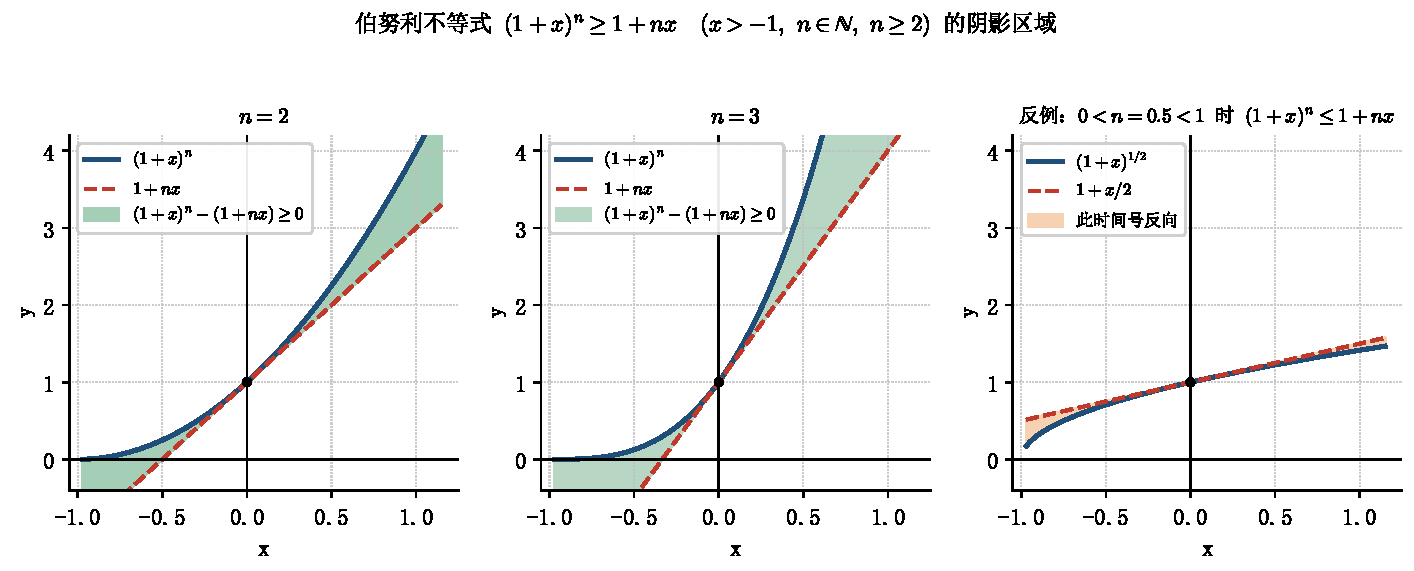
\includegraphics[width=0.99\textwidth]{figures/fig3_bernoulli.pdf}
  \caption{伯努利不等式。左两图 $n=2,3$：阴影区为 $(1+x)^n-(1+nx)\ge0$，
           可见对一切 $x>-1$ 阴影都在上方，且在 $x=0$ 处两者相切（取等）。
           右图为反例对照：$0<n<1$ 时不号反向，说明 $n\in\N,n\ge2$ 的条件不可省。}
  \label{fig:bernoulli}
\end{figure}

\begin{proof}[证明一（归纳法）]
$n=1$ 时两边相等，结论成立（此时为等式）。设对 $n$ 成立，则因 $1+x>0$，
\[
  (1+x)^{n+1}=(1+x)^{n}(1+x)\ \ge\ (1+nx)(1+x)
  =1+(n+1)x+nx^{2}\ \ge\ 1+(n+1)x .
\]
最后一步用到 $nx^2\ge0$。等号需要 $(1+x)^n=1+nx$ 且 $nx^2=0$，
于是在 $n\ge1$ 时必须有 $x=0$。
\end{proof}

\begin{proof}[证明二（二项式展开，直接可见“为什么”）]
\[
  (1+x)^{n}=\sum_{k=0}^{n}\binom{n}{k}x^{k}
  =\underbrace{1}_{k=0}+\underbrace{nx}_{k=1}
   +\underbrace{\sum_{k=2}^{n}\binom{n}{k}x^{k}}_{\ge 0\ \text{（当 }x\ge0\text{）}} .
\]
当 $x\ge0$ 时尾项显然非负。当 $-1<x<0$ 时尾项符号不明，但可以逐项配对处理：
对偶数 $n$，把 $k$ 与 $n-k$ 配对；更简洁的做法是上面的归纳法。
另一个漂亮的论证是：函数 $f(x)=(1+x)^n-(1+nx)$ 满足 $f(0)=0$ 且
$f'(x)=n\big[(1+x)^{n-1}-1\big]$，当 $x>0$ 时 $f'>0$，当 $-1<x<0$ 时
（$n\ge2$ 时 $(1+x)^{n-1}<1$）$f'<0$。故 $x=0$ 是 $f$ 的\emph{全局最小值点}，
$f(x)\ge f(0)=0$。
\end{proof}

\begin{remark}[用伯努利不等式做估计]
由 \eqref{eq:bernoulli} 取 $x=1/n$ 得
$\big(1+\frac1n\big)^n\ge 2$；取 $x=-1/n$（需 $n>1$）得
$\big(1-\frac1n\big)^n\ge 1-n\cdot\frac1n=0$，这个界太松。
更常用的是反向的
\[
  \Big(1+\frac1n\Big)^{n}\le \frac{1}{1-\frac{1}{n+1}}
  =\frac{n+1}{n},
\]
它与 $\big(1+\frac1n\big)^n<e$ 一起构成数列 $a_n=\big(1+\frac1n\big)^n$ 单调有界的经典证明，
见 \S 2.4 中的例（递推数列单调有界）与 \S 1.9。
\end{remark}

% ------------------------------------------------------------------
\subsection{对数与指数不等式}

\begin{theorem}[切线型不等式]\label{thm:logexp}
对一切 $x>0$ 有
\begin{equation}\label{eq:ln}
  \ln x\ \le\ x-1,
\end{equation}
等号当且仅当 $x=1$；对一切 $x\in\R$ 有
\begin{equation}\label{eq:exp}
  e^{x}\ \ge\ 1+x,
\end{equation}
等号当且仅当 $x=0$。更精细地，对一切 $x>0$：
\begin{equation}\label{eq:ln-fine}
  \frac{x}{1+x}\ \le\ \ln(1+x)\ \le\ x .
\end{equation}
\end{theorem}

\begin{figure}[H]
  \centering
  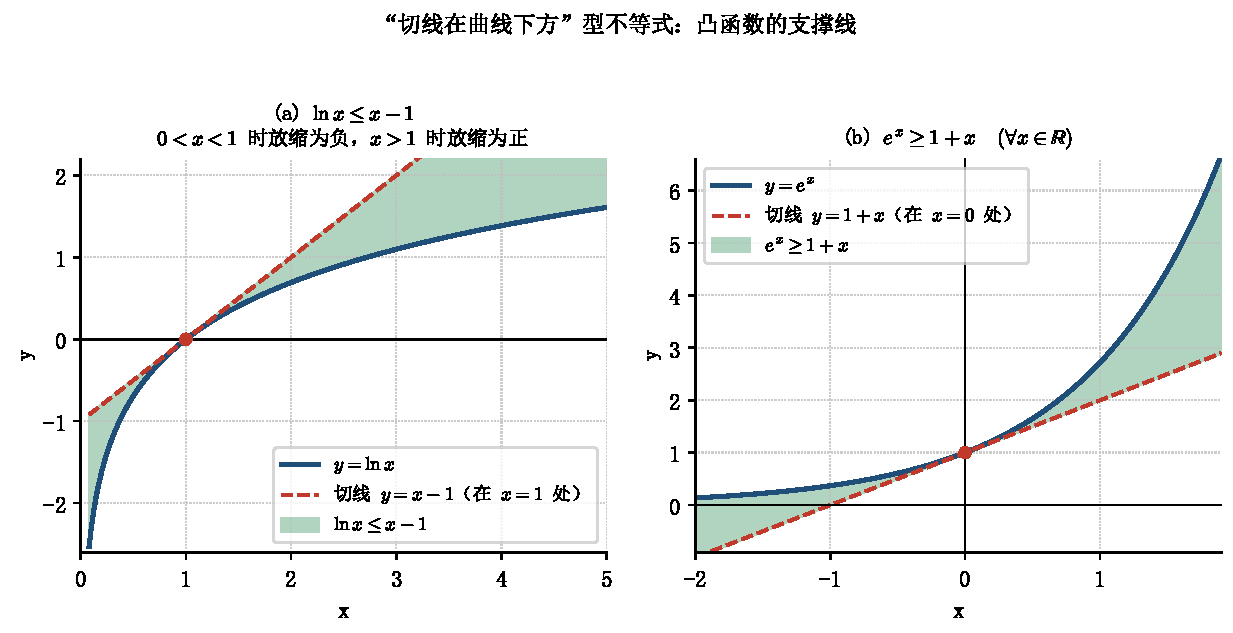
\includegraphics[width=0.96\textwidth]{figures/fig4_tangent.pdf}
  \caption{切线型不等式。$\ln x$ 与 $e^x$ 都是凸函数，其图像位于任一点的切线之上。
           (a) 在 $x=1$ 处的切线为 $y=x-1$，阴影为 $\ln x\le x-1$；
           (b) 在 $x=0$ 处的切线为 $y=1+x$，阴影为 $e^x\ge 1+x$。
           注意 (a) 中 $0<x<1$ 时右端为负、$x>1$ 时右端为正，这在放缩时决定“放缩方向”。}
  \label{fig:tangent}
\end{figure}

\begin{proof}
\emph{(i) 证 $\ln x\le x-1$。} 令 $f(x)=x-1-\ln x$（$x>0$），则
\[
  f'(x)=1-\frac1x=\frac{x-1}{x}.
\]
故 $f$ 在 $(0,1)$ 上单调减、在 $(1,+\infty)$ 上单调增，$x=1$ 为最小值点，
$f(1)=0$。因此 $f(x)\ge0$，即 $\ln x\le x-1$。

\emph{(ii) 证 $e^x\ge1+x$。} 令 $g(x)=e^x-1-x$，则 $g'(x)=e^x-1$，
$g(0)=0$，$g$ 在 $x<0$ 时减、$x>0$ 时增，故 $g(x)\ge g(0)=0$。

\emph{(iii) 证 $\frac{x}{1+x}\le\ln(1+x)\le x$。} 在 (i) 中把 $x$ 换成 $1+x>1$
得 $\ln(1+x)\le x$。在 (i) 中把 $x$ 换成 $\frac{1}{1+x}$ 得
\[
  \ln\frac{1}{1+x}\le \frac{1}{1+x}-1=-\frac{x}{1+x}
  \quad\Longrightarrow\quad
  \ln(1+x)\ \ge\ \frac{x}{1+x}.
\]
注意这一步要求 $\frac{1}{1+x}>0$，即 $x>-1$，与前提 $x>0$ 相容。
\end{proof}

\begin{keybox}[对数不等式的放缩用法]
\eqref{eq:ln-fine} 是\emph{双向}夹逼，因此在估计 $\ln$ 时非常有用。取 $x=1/n$：
\[
  \frac{1}{n+1}\ \le\ \ln\Big(1+\frac1n\Big)\ \le\ \frac1n
  \qquad\Longrightarrow\qquad
  \sum_{k=1}^{n}\frac{1}{k+1}\ \le\ \ln(n+1)\ \le\ \sum_{k=1}^{n}\frac1k .
\]
这直接给出调和级数 $\sum\frac1n$ 与 $\ln n$ 同阶：
$H_n\sim\ln n$（更精确地 $H_n=\ln n+\gamma+o(1)$）。这是\emph{积分放缩}与
\emph{对数放缩}配合的经典范例。
\end{keybox}

% ------------------------------------------------------------------
\subsection{三角函数与 Taylor 型不等式}

\begin{theorem}[基本三角不等式]\label{thm:trig}
\begin{enumerate}[label=(\roman*)]
  \item 对一切 $x\in\R$：$\abs{\sin x}\le\abs{x}$，等号 $\iff x=0$。
  \item 对 $x\in\big(0,\frac{\pi}{2}\big)$：$\sin x<x<\tan x$。
  \item 对 $x\in\big[-\frac{\pi}{2},\frac{\pi}{2}\big]$：$\cos x\ge 1-\frac{x^{2}}{2}$。
  \item 对 $x\in[-1,1]$：$\cos x\le 1-\frac{x^{2}}{2}+\frac{x^{4}}{24}$。
\end{enumerate}
\end{theorem}

\begin{figure}[H]
  \centering
  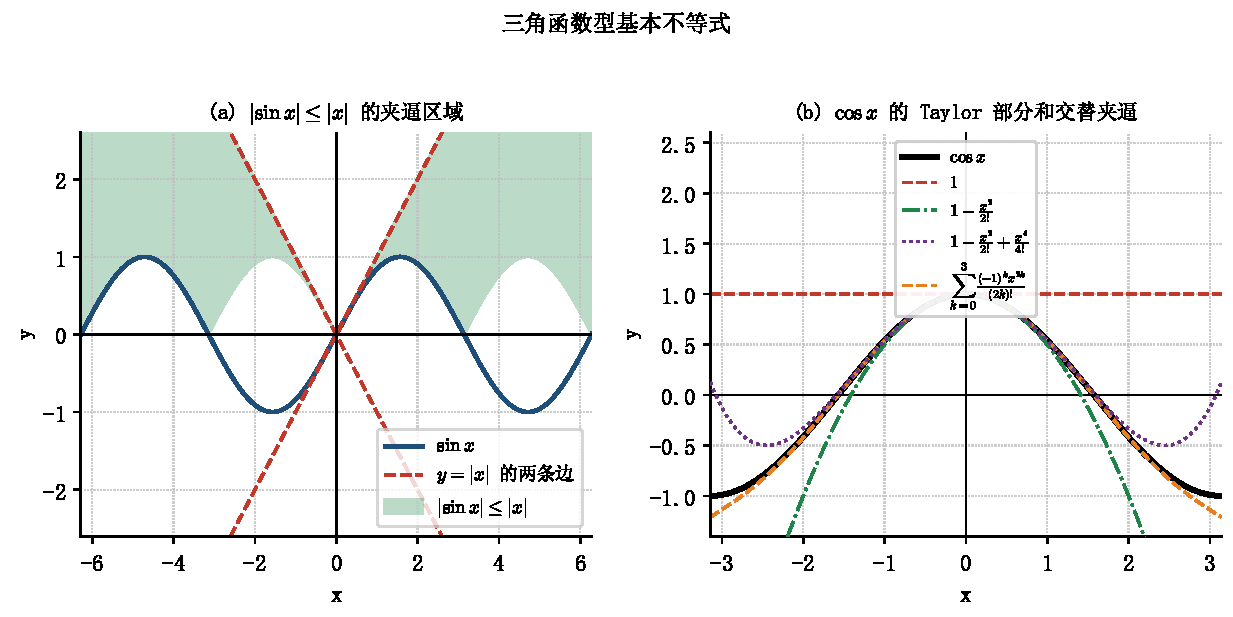
\includegraphics[width=0.96\textwidth]{figures/fig5_sin.pdf}
  \caption{(a) $\abs{\sin x}\le\abs{x}$：正弦曲线被两条直线 $y=\pm x$ 包住，两侧阴影即为两者之间的“余量”。
           (b) $\cos x$ 的 Taylor 部分和 $S_0,S_1,S_2,S_3$ 交替从两侧逼近 $\cos x$，
           偶数阶部分和在下方、奇数阶在上方，这就是“交替级数”的几何来源。}
  \label{fig:sin}
\end{figure}

\begin{proof}
\emph{(i)} 由奇偶性只需证 $x\ge0$。令 $f(x)=x-\sin x$，$f(0)=0$，
$f'(x)=1-\cos x\ge0$，故 $f$ 单调不减，$f(x)\ge0$。等号只在 $x=0$（因为
$f$ 在 $(0,+\infty)$ 上严格增）。

\emph{(ii)} $\sin x<x$ 即 (i)。对 $x<\tan x$，令 $g(x)=\tan x-x$，
$g(0)=0$，$g'(x)=\sec^2x-1=\tan^2x>0$（$x\in(0,\pi/2)$），故 $g>0$。

\emph{(iii)} 令 $h(x)=\cos x-1+\frac{x^2}{2}$，则
$h(0)=0$，$h'(x)=-\sin x+x\overset{\text{(i)}}{\ge}0$，故 $h(x)\ge0$。

\emph{(iv)} 令 $k(x)=1-\frac{x^2}{2}+\frac{x^4}{24}-\cos x$，则
$k(0)=0$，$k'(x)=-x+\frac{x^3}{6}+\sin x$，$k'(0)=0$，
$k''(x)=-1+\frac{x^{2}}{2}+\cos x=-(1-\cos x)+\frac{x^2}{2}$。
由 (iii)（$1-\cos x\le\frac{x^2}{2}$）得 $k''(x)\ge0$，于是 $k'$ 单增、
$k'\ge k'(0)=0$，于是 $k$ 单增、$k\ge k(0)=0$。
\end{proof}

\begin{remark}[Taylor 余项的统一视角]
(i)(iii)(iv) 都可以看成 Taylor 公式的\emph{带符号余项}：对
\[
  \sin x=\sum_{k\ge0}\frac{(-1)^{k}x^{2k+1}}{(2k+1)!},
  \qquad
  \cos x=\sum_{k\ge0}\frac{(-1)^{k}x^{2k}}{(2k)!},
\]
\emph{截断在任意偶数/奇数阶}都给出有确定符号的余项。这样得到的界不仅有方向，
而且\emph{可以随时“加一项”来收紧}，是放缩法中“可迭代收紧”的典范。
\end{remark}

% ------------------------------------------------------------------
\subsection{积分不等式}

\begin{theorem}[积分放缩的基本工具]\label{thm:integral}
设 $f$ 在 $[a,b]$ 上可积。
\begin{enumerate}[label=(\roman*)]
  \item \textbf{保序性}：若 $f(x)\le g(x)$ 对一切 $x\in[a,b]$ 成立，则
        $\displaystyle\int_a^b f\le\int_a^b g$。
  \item \textbf{估值定理}：若 $m\le f\le M$，则
        $\displaystyle m(b-a)\le\int_a^b f\le M(b-a)$。
  \item \textbf{绝对值不等式}：$\displaystyle\abs{\int_a^b f}\le\int_a^b\abs f$。
  \item \textbf{积分中值定理}：$f$ 连续时存在 $\xi\in[a,b]$ 使
        $\displaystyle\int_a^b f=f(\xi)(b-a)$。
\end{enumerate}
\end{theorem}

\begin{figure}[H]
  \centering
  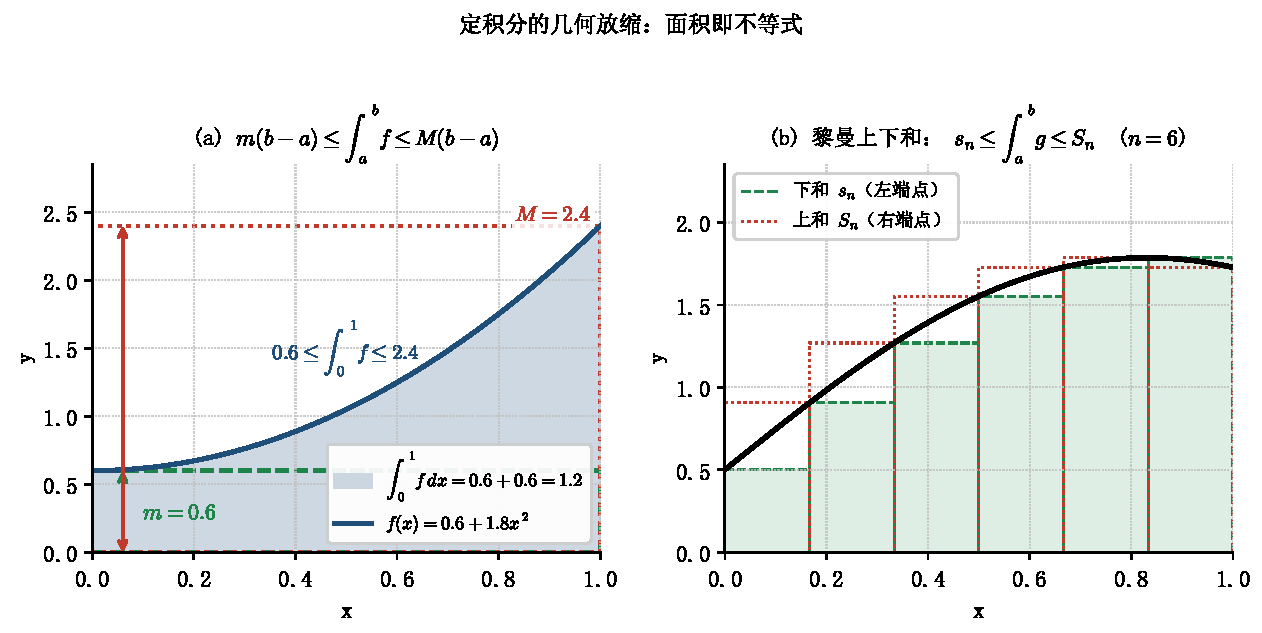
\includegraphics[width=0.96\textwidth]{figures/fig7_integral.pdf}
  \caption{(a) 估值定理的“面积”含义：曲线下方的面积 $\int_0^1f=1.2$ 被夹在
           内接宽矩形 $m(b-a)=0.6$ 与外接高矩形 $M(b-a)=2.4$ 之间。
           (b) 黎曼上下和：$n=6$ 时下和 $s_n$（左端点矩形）$\le\int_0^1 g\le$ 上和 $S_n$（右端点矩形）；
           $n\to\infty$ 时两串矩形同时挤压曲线下方区域。}
  \label{fig:integral}
\end{figure}

\begin{theorem}[Hermite–Hadamard 不等式]\label{thm:hh}
设 $f$ 在 $[a,b]$ 上连续且为凸函数，则
\begin{equation}\label{eq:hh}
  f\Big(\frac{a+b}{2}\Big)\ \le\ \frac{1}{b-a}\int_a^b f(x)\dd x
  \ \le\ \frac{f(a)+f(b)}{2}.
\end{equation}
\end{theorem}

\begin{figure}[H]
  \centering
  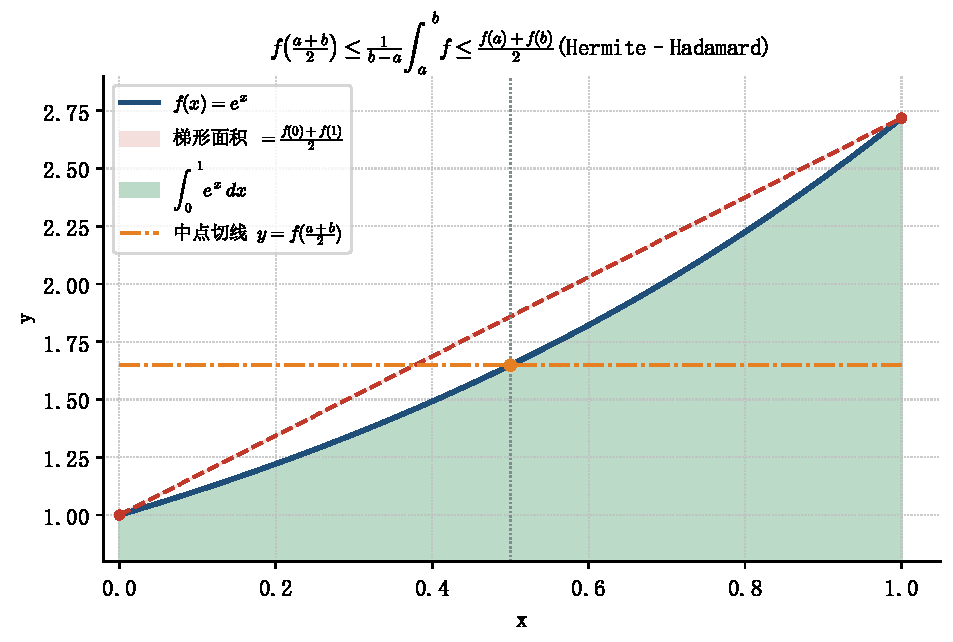
\includegraphics[width=0.75\textwidth]{figures/fig6_hermite.pdf}
  \caption{Hermite–Hadamard 不等式的面积图像（以 $f(x)=e^x$ 为例）：
           积分 $\int_0^1e^x\dd x=e-1\approx1.718$ 介于
           中点处高度（$e^{1/2}\approx1.649$）与梯形平均高度（$\approx1.859$）之间。}
  \label{fig:hh}
\end{figure}

\begin{proof}
\textbf{右半部分}：由 $f$ 凸，图像位于弦\emph{下方}，即
\[
  f\big((1-t)a+tb\big)\ \le\ (1-t)f(a)+tf(b),\qquad t\in[0,1].
\]
作代换 $x=(1-t)a+tb$，$\dd x=(b-a)\dd t$，对 $t$ 从 $0$ 到 $1$ 积分：
\[
  \int_a^bf(x)\dd x=(b-a)\int_0^1f\big((1-t)a+tb\big)\dd t
  \le(b-a)\int_0^1\big[(1-t)f(a)+tf(b)\big]\dd t
  =(b-a)\cdot\frac{f(a)+f(b)}{2}.
\]

\textbf{左半部分}：令 $c=\frac{a+b}{2}$，$s\in[0,1]$，取对称点 $c-s$ 与 $c+s$。由凸性
\[
  f(c)=f\Big(\frac{(c-s)+(c+s)}{2}\Big)\ \le\ \frac{f(c-s)+f(c+s)}{2}.
\]
两边对 $s$ 在 $[0,1]$ 上积分。注意 $s\in[0,1]$ 对应 $x\in[a,c]$ 与 $[c,b]$ 的对称遍历，
\[
  \int_0^1\frac{f(c-s)+f(c+s)}{2}\dd s
  =\frac{1}{2}\Big(\int_{a}^{c}f+\int_c^{b}f\Big)\cdot\frac{2}{b-a}
  =\frac{1}{b-a}\int_a^bf ,
\]
其中代换为 $x=c-s$ 与 $x=c+s$（各自 $\dd x=\mp\dd s$，上下限相应倒置）。
于是 $f(c)\le\frac{1}{b-a}\int_a^bf$。
\end{proof}

% ------------------------------------------------------------------
\subsection{Young 不等式}

\begin{theorem}[Young]\label{thm:young}
设 $p,q>1$ 满足 $\frac1p+\frac1q=1$（称共轭指数），$a,b\ge0$，则
\begin{equation}\label{eq:young}
  ab\ \le\ \frac{a^{p}}{p}+\frac{b^{q}}{q},
\end{equation}
等号当且仅当 $a^{p}=b^{q}$。
\end{theorem}

\begin{figure}[H]
  \centering
  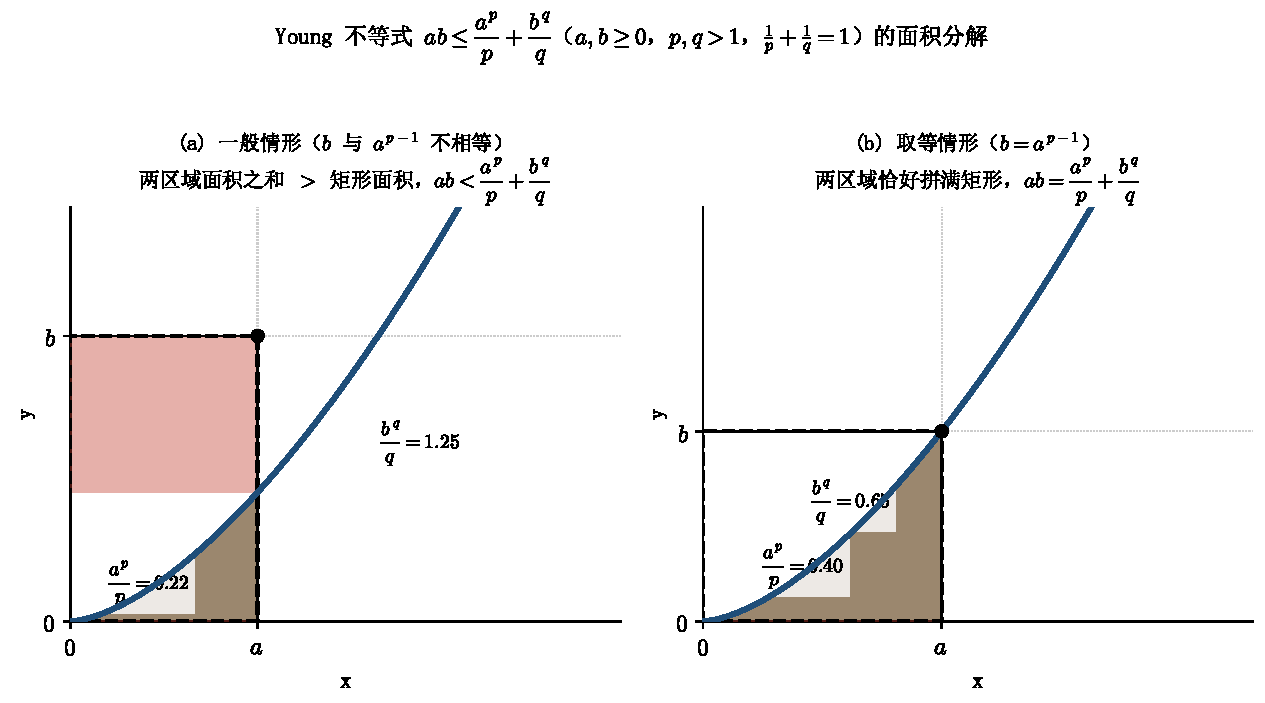
\includegraphics[width=0.92\textwidth]{figures/fig10_young.pdf}
  \caption{Young 不等式的面积分解。取曲线 $f(x)=x^{p-1}$，矩形 $[0,a]\times[0,b]$ 面积为 $ab$。
           曲线下方的绿色区域面积是 $\frac{a^p}{p}$，矩形内其余部分（红色）面积恰为 $\frac{b^q}{q}$
           —— 但注意只有 $b\ge a^{p-1}$ 时红色区域才完整落在矩形内。
           (b) 当 $b=a^{p-1}$（即 $a^p=b^q$）时两区域恰好\emph{互补铺满}矩形，等号成立。}
  \label{fig:young}
\end{figure}

\begin{proof}[证明一（利用 $\ln$ 的凹性）]
当 $a=0$ 或 $b=0$ 时 \eqref{eq:young} 显然成立。设 $a,b>0$，令
$u=\frac{a^{p}}{p}$，$v=\frac{b^{q}}{q}$，$w=\frac{1}{p}$，则 $\frac1q=1-w$。
由 $\ln$ 的凹性（$\ln''x=-1/x^2<0$）与加权 Jensen 不等式：
\[
  \ln\Big(w\cdot a^{p}+(1-w)\cdot b^{q}\Big)
  \ \ge\ w\ln(a^{p})+(1-w)\ln(b^{q})
  =\frac{1}{p}\ln a^p+\frac{1}{q}\ln b^q
  =\ln a+\ln b=\ln(ab).
\]
两边取指数即得 $ab\le\frac{a^p}{p}+\frac{b^q}{q}$。
等号成立当且仅当 $a^{p}=b^{q}$（Jensen 取等条件：两点相同）。
\end{proof}

\begin{proof}[证明二（微积分法，可推广为“用 $b$ 优化”）]
固定 $a>0$，令
\[
  \varphi(b)=\frac{a^{p}}{p}+\frac{b^{q}}{q}-ab,\qquad b\ge0 .
\]
则 $\varphi'(b)=b^{q-1}-a$，唯一临界点 $b_0=a^{\frac{1}{q-1}}$。
由 $\frac1p+\frac1q=1$ 得 $\frac{1}{q-1}=p-1$，故 $b_0=a^{p-1}$，
且 $a^{p}=a\cdot a^{p-1}=ab_0=b_0^{q}$。
$\varphi''(b)=(q-1)b^{q-2}>0$，故 $b_0$ 为最小值点：
\[
  \varphi(b)\ \ge\ \varphi(b_0)
  =\frac{a^{p}}{p}+\frac{b_0^{q}}{q}-ab_0
  =\frac{a^{p}}{p}+\frac{a^{p}}{q}-a^{p}
  =a^{p}\Big(\frac1p+\frac1q-1\Big)=0 .
\]
这就是 \eqref{eq:young}。等号仅在 $b=b_0$，即 $a^p=b^q$。
\end{proof}

\begin{keybox}[Young 不等式的两大用途]
\begin{enumerate}[label=(\arabic*)]
  \item \textbf{导出 Hölder 不等式}：在 \eqref{eq:young} 中代 $a=\frac{u_k}{U}$、
        $b=\frac{v_k}{V}$（其中 $U^{p}=\sum u_k^p$，$V^{q}=\sum v_k^q$）并对 $k$ 求和，
        即得
        \[
          \sum_{k=1}^{n}u_kv_k\ \le\ \Big(\sum u_k^{p}\Big)^{1/p}\Big(\sum v_k^{q}\Big)^{1/q}.
        \]
  \item \textbf{$\eps$-不等式}：取 $p=2$ 得 $ab\le\frac{\eps}{2}a^{2}+\frac{1}{2\eps}b^{2}$，
        这是分析中“吸收小项”的标准手段：给定 $\eps>0$ 可把交叉项压到任意小。
\end{enumerate}
\end{keybox}

% ------------------------------------------------------------------
\subsection{排序不等式与 Chebyshev 不等式}

\begin{theorem}[排序不等式 / 重排不等式]\label{thm:rearrange}
设两组实数均按递增排列：
\[
  a_1\le a_2\le\cdots\le a_n,\qquad b_1\le b_2\le\cdots\le b_n .
\]
对 $\{1,\dots,n\}$ 的任一排列 $\sigma$，有
\begin{equation}\label{eq:rearrange}
  \sum_{i=1}^{n}a_i b_{n+1-i}\ \le\ \sum_{i=1}^{n}a_i b_{\sigma(i)}
  \ \le\ \sum_{i=1}^{n}a_i b_i .
\end{equation}
即：\textbf{同序和 $\ge$ 乱序和 $\ge$ 反序和}。
\end{theorem}

\begin{figure}[H]
  \centering
  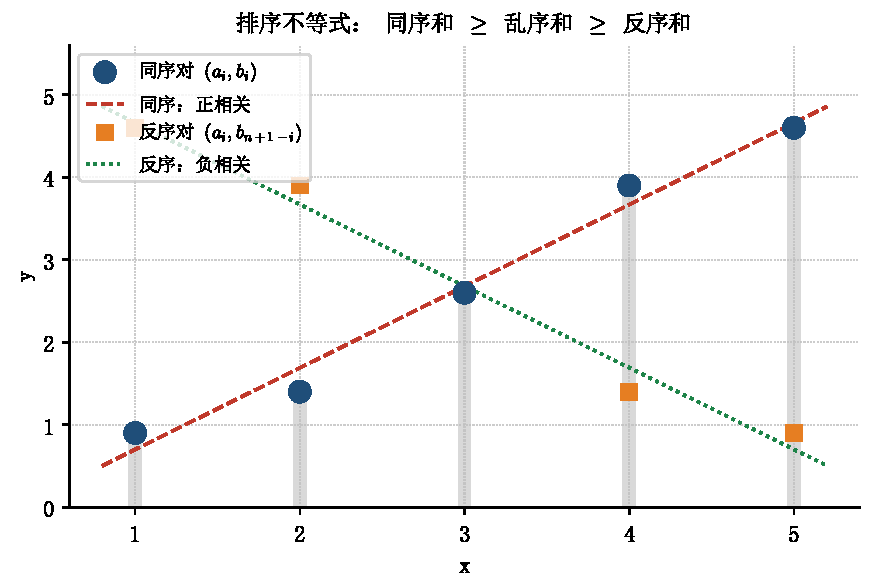
\includegraphics[width=0.72\textwidth]{figures/fig11_chebyshev.pdf}
  \caption{排序不等式的图解。蓝点：同序配对 $(a_i,b_i)$，点列呈上升趋势（正相关），
           乘积和最大；橙方：反序配对 $(a_i,b_{n+1-i})$，点列呈下降趋势（负相关），乘积和最小。}
  \label{fig:rearrange}
\end{figure}

\begin{proof}
只需证“交换一对逆序不减小和”。设 $i<j$ 但 $b_{\sigma(i)}>b_{\sigma(j)}$，
记 $x=b_{\sigma(i)}$，$y=b_{\sigma(j)}$（$x>y$），$a=a_i$，$b=a_j$（$a\le b$）。
比较交换前后的两项：
\[
  \big(ax+by\big)-\big(ay+bx\big)=(a-b)(x-y)\ \le 0,
\]
因为 $a-b\le0$ 而 $x-y>0$。所以交换后和不减。若 $\sigma$ 不是恒等排列，
则存在逆序，逐次交换（每次使和单调不减）最终变为恒等排列，于是
$\sum a_ib_{\sigma(i)}\le\sum a_ib_i$。同理，若 $\sigma$ 不是反序排列，
也可逐次交换使和单调不减，最后达到反序排列，故反序和为最小值。
\end{proof}

\begin{corollary}[Chebyshev 不等式]\label{cor:chebyshev}
若 $a_1\le\cdots\le a_n$，$b_1\le\cdots\le b_n$，则
\begin{equation}\label{eq:chebyshev}
  \frac1n\sum_{i=1}^{n}a_ib_i\ \ge\
  \Big(\frac1n\sum_{i=1}^{n}a_i\Big)\Big(\frac1n\sum_{i=1}^{n}b_i\Big).
\end{equation}
\end{corollary}

\begin{proof}
在 \eqref{eq:rearrange} 中对全部 $n!$ 个排列求和。左边每个 $a_ib_j$ 恰好出现
$(n-1)!$ 次（固定 $i$ 与 $j=\sigma(i)$，其余自由），故
\[
  (n-1)!\sum_{i,j}a_ib_j\ \le\ n!\sum_{i}a_ib_i .
\]
两边除以 $n!$ 并整理得 $n\sum a_ib_i\ge\big(\sum a_i\big)\big(\sum b_i\big)$，
即 \eqref{eq:chebyshev}。
\end{proof}

\begin{warnbox}[常见误用]
Chebyshev 不等式\emph{要求两列同向单调}。若 $a$ 与 $b$ 反序，则不等号方向相反；
若单调性不明，该式一般\emph{不成立}。例如
$a=(1,3)$，$b=(3,1)$：$a_1b_1+a_2b_2=6$，
而 $\frac12(\sum a)(\sum b)=\frac12\cdot4\cdot4=8>6$。
\end{warnbox}

% ------------------------------------------------------------------
\subsection{夹逼定理与数列的常用界}

\begin{theorem}[夹逼定理]\label{thm:squeeze}
\begin{enumerate}[label=(\roman*)]
  \item \textbf{数列}：若存在 $N$ 使得对一切 $n\ge N$ 有
        $x_n\le y_n\le z_n$，且 $\lim x_n=\lim z_n=A$，则 $\lim y_n=A$。
  \item \textbf{函数}：若 $g(x)\le f(x)\le h(x)$ 在 $x_0$ 的某去心邻域内成立，
        且 $\lim_{x\to x_0}g=\lim_{x\to x_0}h=A$，则 $\lim_{x\to x_0}f=A$。
\end{enumerate}
\end{theorem}

\begin{figure}[H]
  \centering
  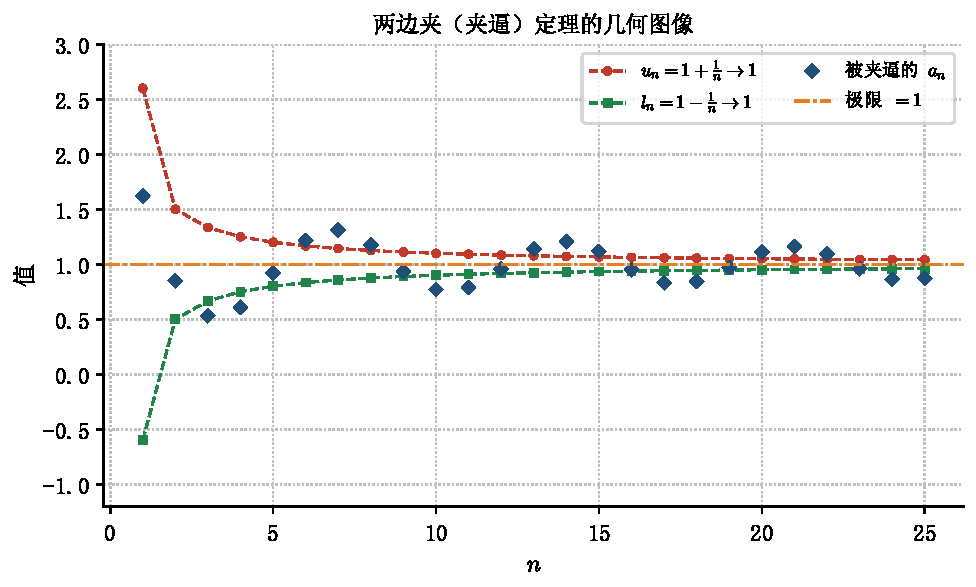
\includegraphics[width=0.78\textwidth]{figures/fig12_squeeze_seq.pdf}
  \caption{夹逼定理的几何图像。上界 $u_n=1+\frac1n$ 与下界 $l_n=1-\frac1n$ 从两侧向 $1$ 收缩，
           被夹逼的 $a_n=1+\frac{\cos(0.9n)}{n^{0.6}}$ 始终落在两者之间，因而必然收敛到 $1$。}
  \label{fig:squeezeseq}
\end{figure}

\begin{proof}
只证 (i)。设 $\eps>0$。由 $\lim x_n=A$ 与 $\lim z_n=A$，存在 $N_1,N_2$ 使
$n\ge N_1$ 时 $\abs{x_n-A}<\eps$，$n\ge N_2$ 时 $\abs{z_n-A}<\eps$。
取 $N_0=\max\{N,N_1,N_2\}$，对 $n\ge N_0$ 有
\[
  A-\eps<x_n\le y_n\le z_n<A+\eps
  \quad\Longrightarrow\quad \abs{y_n-A}<\eps .
\]
按定义 $y_n\to A$。
\end{proof}

\begin{keybox}[必须记住的常数极限]
\begin{align*}
  &\lim_{n\to\infty}\Big(1+\frac1n\Big)^{n}=e, &
  &\lim_{n\to\infty}\sqrt[n]{n}=1, \\
  &\lim_{n\to\infty}\frac{\ln n}{n}=0, &
  &\lim_{n\to\infty}\frac{a^{n}}{n!}=0\quad(\forall a>0), \\
  &\lim_{n\to\infty}\sqrt[n]{a}=1\quad(a>0), &
  &\lim_{x\to0}\frac{\sin x}{x}=1,\qquad
   \lim_{x\to0}\frac{\ln(1+x)}{x}=1 .
\end{align*}
\end{keybox}

\newpage

% ============================ 第 2 章 ============================
\section{放缩法的方法论}

前面把“武器”备齐了，这一章讨论“怎么用”。放缩的手法虽然繁多，但归纳起来不外乎
\begin{center}
\fbox{\parbox{0.86\linewidth}{\centering
\textbf{逐项放缩 $|$ 裂项放缩 $|$ 积分放缩 $|$ 单调性放缩 $|$ 切线放缩 $|$ 分情况放缩}}}
\end{center}
下面逐一说明每种手法的\emph{适用场景}与\emph{关键技巧}。

% ------------------------------------------------------------------
\subsection{第一范式：逐项放缩（把每项换成更简单的一项）}

\textbf{思想}：和式（或积式）中每项结构复杂，但若能证明“第 $k$ 项 $\le$ 某个简单式子”，
就得到整体界。关键是\emph{同一化}：让各项共用同一分母、同一形式。

\begin{example}[统一分母]
证明 $\displaystyle\sum_{k=1}^{n}\frac{1}{n^{2}+k}\ \le\ \frac{1}{n}$（$n\ge1$）。
\end{example}

\begin{proof}
每项的分母 $n^2+k\ge n^2$，故 $\frac{1}{n^2+k}\le\frac{1}{n^2}$。共 $n$ 项：
\[
  \sum_{k=1}^{n}\frac{1}{n^{2}+k}\ \le\ n\cdot\frac{1}{n^{2}}=\frac1n .
\]
\end{proof}

\begin{warnbox}[逐项放缩的陷阱：项数与精度会“打架”]
上例中界 $1/n$ 已经最优（因为最大项本身就 $\approx 1/n^2$，
但项数为 $n$，且各项都接近 $1/n^2$，所以总和 $\approx n\cdot\frac{1}{n^2}=\frac1n$）。
但如果放缩成 $\frac{1}{n^2+k}\le\frac{1}{k}$，求和得 $H_n$，界就比真值大 $\ln n$ 倍，
\emph{完全失效}。
\par\smallskip
\textbf{教训}：逐项放缩时必须保证\emph{每一项的放缩误差同阶}，
否则误差会累积并淹没主项。
\end{warnbox}

\begin{example}[奇偶配对放缩]\label{ex:odd-even}
证明 $\displaystyle\sum_{k=1}^{2n}(-1)^{k}\frac{1}{k}$ 收敛。
\end{example}

\begin{proof}
令 $b_k=\frac{1}{k}$ 单调递减趋零。将相邻两项配对：
\[
  \sum_{k=1}^{2n}(-1)^{k}\frac1k
  =-\Big(\frac11-\frac12\Big)-\Big(\frac13-\frac14\Big)-\cdots-\Big(\frac{1}{2n-1}-\frac{1}{2n}\Big).
\]
每对括号内均为正，故部分和为负且递减。又
\[
  \abs{\sum_{k=1}^{2n}(-1)^{k}\frac1k}\ \le\ \frac{1}{1}=1
\]
（Leibniz 型估计：交错级数的和介于任意两相邻部分和之间，故 $\le b_1$）。
于是偶子列单调有界故收敛；奇子列与偶子列只差一项 $\frac{1}{2n+1}\to0$，
故同收敛于同一点。
\end{proof}

\begin{figure}[H]
  \centering
  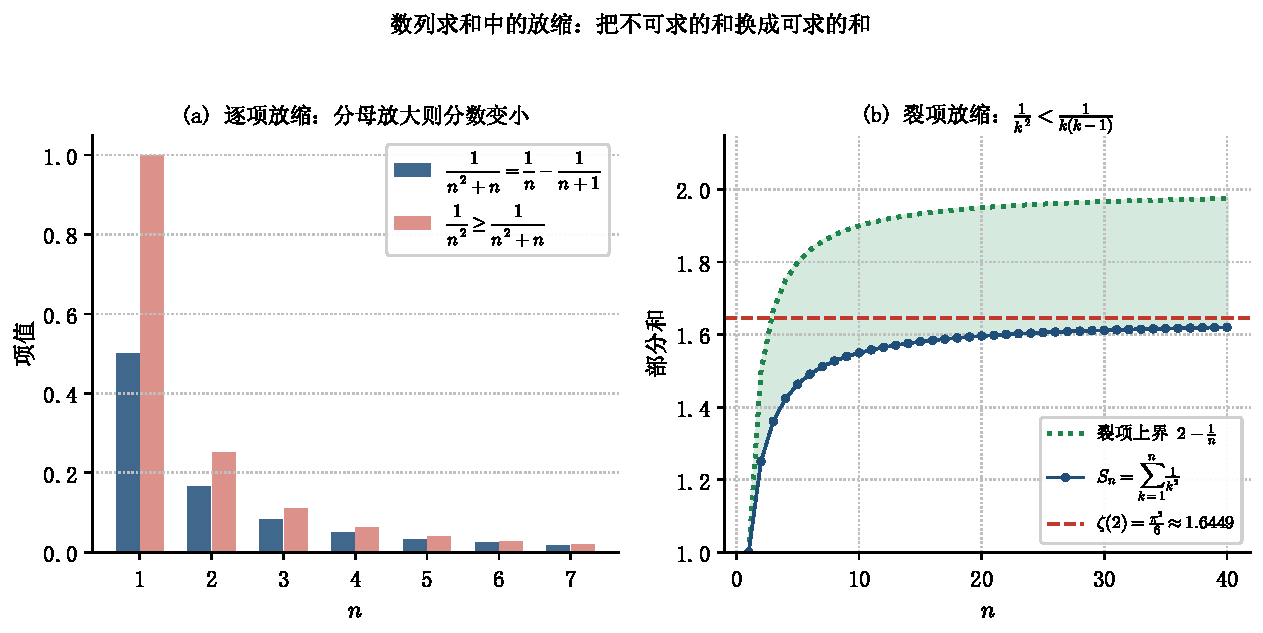
\includegraphics[width=0.96\textwidth]{figures/fig9_sum_bound.pdf}
  \caption{(a) 逐项放缩的核心：分母“放大”则分数“缩小”。
           $\frac{1}{n^2}\ge\frac{1}{n^2+n}=\frac1n-\frac1{n+1}$ 把不可裂项的 $1/n^2$ 换成了可裂项表达式。
           (b) 由此得到 $\sum_{k=1}^n\frac1{k^2}\le 2-\frac1n<2$，
           实线部分和 $S_n$ 始终位于点线上界之下，且上界本身有界，故级数收敛；
           图中另标出真值 $\zeta(2)=\pi^2/6\approx1.6449$。}
  \label{fig:sumbound}
\end{figure}

% ------------------------------------------------------------------
\subsection{第二范式：裂项放缩（把求和换成首尾之差）}

\textbf{思想}：若能找到 $t_k$ 使第 $k$ 项 $\le t_k-t_{k+1}$，则 $\sum$ 自动裂项、边界项抵消。
这通常是处理“分母为二次式”的求和题的首选。

\begin{keybox}[三个必背裂项式]
{\small
\begin{align*}
  \frac{1}{k(k+1)}&=\frac1k-\frac{1}{k+1},\\[2pt]
  \frac{1}{k(k-1)}&=\frac{1}{k-1}-\frac1k\qquad(k\ge2),\\[2pt]
  \frac{1}{k(k+1)(k+2)}&=\frac12\Big[\frac{1}{k(k+1)}-\frac{1}{(k+1)(k+2)}\Big].
\end{align*}}
以上三式均为\emph{等式}；配合“放缩成二次分母”即可把级数收敛性、求和估计一并解决。
\end{keybox}

\begin{example}[级数收敛性的裂项证明]\label{ex:series}
证明 $\displaystyle\sum_{n=1}^{\infty}\frac{1}{n^{2}}$ 收敛，且其和 $<2$。
\end{example}

\begin{proof}
对 $k\ge1$ 有 $k^2+k>k^2$，故
\[
  \frac{1}{k^{2}}\ >\ \frac{1}{k^{2}+k}=\frac1k-\frac{1}{k+1}.
\]
但这个方向给出的是\emph{下界}：$\sum\frac1{k^2}>\sum\big(\frac1k-\frac1{k+1}\big)=1-\frac{1}{n+1}$，
只能说明 $S_n>1-\frac1{n+1}$，不足以证明收敛（下界不能说明有界）。

要用裂项法证明\emph{收敛}，必须控制住\emph{上界}。正确做法是只对 $k\ge2$ 放缩：
当 $k\ge2$ 时 $k^{2}>k(k-1)=k^2-k$，故
\[
  \frac{1}{k^{2}}\ <\ \frac{1}{k(k-1)}=\frac{1}{k-1}-\frac1k\qquad(k\ge2).
\]
于是
\[
  S_n=\underbrace{1}_{k=1}+\sum_{k=2}^{n}\frac{1}{k^{2}}
  \ <\ 1+\sum_{k=2}^{n}\Big(\frac{1}{k-1}-\frac1k\Big)
  =1+\Big(1-\frac1n\Big)=2-\frac1n\ <\ 2 .
\]
$S_n$ 单调递增（各项为正）且有上界 $2$，故收敛，且和 $\le 2$。
\end{proof}

\begin{warnbox}[方向检查：这是最容易出错的一步]
上面两次尝试的差别只有\emph{一个不等号方向}和\emph{一个下标}：
\[
  \underbrace{\frac{1}{k^2}>\frac{1}{k(k+1)}}_{\text{给出下界，无用}}
  \qquad\text{vs.}\qquad
  \underbrace{\frac{1}{k^2}<\frac{1}{k(k-1)}\ (k\ge2)}_{\text{给出上界，有用}}.
\]
写裂项放缩时，请先问自己：“我需要的是\emph{上界}还是\emph{下界}？”
\end{warnbox}

\begin{tipbox}[“保留首项、尾巴放缩”的通用套路]
凡遇到“分子为常数、分母为多项式”的求和估计，标准动作是：
\begin{enumerate}[label=\arabic*.]
  \item 先算出\emph{前几项}（通常是 1--2 项）作为\emph{主要部分}保留原样；
  \item 对于余下的项，把分母\emph{放大或缩小}成\emph{可裂项}的形式；
  \item 裂项求和，得到与 $n$ 有关的界，考察其极限。
\end{enumerate}
如果直接对首项也放缩，往往会\emph{得到错误的方向}（如上面 Remark 所示）。
\end{tipbox}

% ------------------------------------------------------------------
\subsection{第三范式：积分放缩（用面积替代求和）}

\textbf{思想}：若 $f$ 单调，则 $\sum f(k)$ 与 $\int f$ 只差一个\emph{首尾项}。
这在估计 $H_n$、$\ln n!$、判别级数敛散性时极为常用。

\begin{theorem}[积分判别法]\label{thm:integral-test}
设 $f:[1,+\infty)\to[0,+\infty)$ 连续、单调递减。则
\begin{equation}\label{eq:integral-bound}
  \int_1^{n+1}f(x)\dd x\ \le\ \sum_{k=1}^{n}f(k)\ \le\ f(1)+\int_1^{n}f(x)\dd x .
\end{equation}
特别地，$\sum f(k)$ 收敛 $\iff$ $\int_1^\infty f$ 收敛。
\end{theorem}

\begin{proof}
对每个 $k\ge1$，由 $f$ 在 $[k,k+1]$ 上单调递减，有
\[
  f(k+1)\ \le\ f(x)\ \le\ f(k)\qquad(x\in[k,k+1]).
\]
在 $[k,k+1]$ 上积分（区间长度为 $1$）：
\begin{equation}\label{eq:int-test-1}
  f(k+1)\ \le\ \int_k^{k+1}f(x)\dd x\ \le\ f(k).
\end{equation}

\textbf{下界}：把 \eqref{eq:int-test-1} 的右半（$\int_k^{k+1}f\le f(k)$）对
$k=1,2,\dots,n$ 求和，得
\[
  \int_1^{n+1}f(x)\dd x=\sum_{k=1}^{n}\int_k^{k+1}f(x)\dd x
  \ \le\ \sum_{k=1}^{n}f(k).
\]

\textbf{上界}：把 \eqref{eq:int-test-1} 的左半（$f(k+1)\le\int_k^{k+1}f$）对
$k=1,2,\dots,n-1$ 求和，得
\[
  \sum_{k=2}^{n}f(k)\ \le\ \int_1^{n}f(x)\dd x,
\]
两边加上 $f(1)$ 即得 $\displaystyle\sum_{k=1}^{n}f(k)\le f(1)+\int_1^{n}f$。

合起来就是 \eqref{eq:integral-bound}。由于 $f\ge0$，右端关于 $n$ 单调增，
于是“$\sum f(k)$ 有界 $\iff$ $\int_1^\infty f$ 收敛”。
\end{proof}

\begin{example}[调和级数的对数渐近]\label{ex:harmonic}
证明 $\ln(n+1)\le H_n\le 1+\ln n$，其中 $H_n=\sum_{k=1}^{n}\frac1k$。
\end{example}

\begin{proof}
取 $f(x)=1/x$ 代入 \eqref{eq:integral-bound}：
\[
  \int_1^{n+1}\frac{\dd x}{x}=\ln(n+1)\ \le\ H_n\ \le\ 1+\int_1^{n}\frac{\dd x}{x}=1+\ln n .
\]
\end{proof}

\begin{corollary}[Stirling 型估计]
$\ln(n!)=\sum_{k=1}^{n}\ln k$ 介于
$\int_1^{n+1}\ln x\dd x$ 与 $\ln 1+\int_1^n\ln x\dd x$ 之间，
化简得
\[
  n\ln n-n+1\ \le\ \ln(n!)\ \le\ (n+1)\ln(n+1)-n ,
\]
即 $n!\approx\big(\frac ne\big)^n$ 的量级。
\end{corollary}

% ------------------------------------------------------------------
\subsection{第四范式：单调性放缩（构造函数、求导定界）}

\textbf{思想}：要证 $A(x)\ge B(x)$，令 $F=A-B$，证明 $F$ 的最小值 $\ge0$。
这是\S 1.4 全部证明的通用骨架，也是“切线型不等式”的来源。

\begin{example}[递推数列的单调有界]\label{ex:recursion}
设 $a_1=\sqrt2$，$a_{n+1}=\sqrt{2+a_n}$。证明 $\{a_n\}$ 收敛并求极限。
\end{example}

\begin{proof}
\textbf{有界性}：先归纳证明 $a_n<2$。$a_1=\sqrt2<2$；若 $a_n<2$，则
$a_{n+1}=\sqrt{2+a_n}<\sqrt{2+2}=2$。

\textbf{单调性}：考察
\[
  a_{n+1}-a_n=\sqrt{2+a_n}-a_n .
\]
令 $x=a_n\in(0,2)$，则 $\sqrt{2+x}-x$ 的符号：$\sqrt{2+x}\ge x$
$\iff 2+x\ge x^2\iff x^2-x-2\le0\iff -1\le x\le2$，在 $x\in(0,2)$ 上成立。
故 $a_{n+1}\ge a_n$，即数列单调增。

\textbf{求极限}：单调增且有上界 $2$，故收敛，设极限为 $L$。在递推式两边取极限
（利用 $\sqrt{\cdot}$ 的连续性与 $L\ge\sqrt2>0$）得 $L=\sqrt{2+L}$，即
$L^2-L-2=0$，$L=2$ 或 $L=-1$。因 $L\ge a_1>0$，故 $L=2$。
\end{proof}

\begin{example}[$\big(1+\frac1n\big)^n$ 的收敛性]
$b_n=\big(1+\frac1n\big)^{n}$ 单调递增且 $b_n<3$。
\end{example}

\begin{proof}[要点]
\textbf{上界}：由二项式展开
\[
  b_n=\sum_{k=0}^{n}\binom nk\frac{1}{n^{k}}
  \le\sum_{k=0}^{n}\frac{1}{k!}
  \le 1+1+\frac12+\frac14+\cdots=3,
\]
第一处不等号用到 $\binom nk/n^k=\frac{1}{k!}\prod_{j=0}^{k-1}\big(1-\frac jn\big)\le\frac{1}{k!}$，
第二处用到 $k!\ge2^{k-1}$（$k\ge1$）。

\textbf{单调增}：把 $b_n$ 写成 $b_n=\sum_{k=0}^{n}\frac{1}{k!}\prod_{j=0}^{k-1}\big(1-\frac jn\big)$，
每一个因子 $\big(1-\frac jn\big)$ 都关于 $n$ 递增，且 $n$ 增大时末尾还多出正项，
故 $b_n\le b_{n+1}$。于是 $b_n\to e$。
\end{proof}

% ------------------------------------------------------------------
\subsection{第五范式：切线放缩（用线性函数包住非线性函数）}

\textbf{思想}：若 $f$ 凸，则任一点的切线都在图像\emph{下方}；若 $f$ 凹，切线在\emph{上方}。
因此可以用切线（简单、可求和）替代原函数。\S 1.4 的 \eqref{eq:ln}, \eqref{eq:exp} 就是这一范式的产物。

\begin{keybox}[切线放缩的三个常用模板]
\[
  \ln x\le x-1,\qquad e^{x}\ge1+x,\qquad
  \frac{1}{1+x}\ge 1-x\quad(\abs x<1).
\]
第三式由 $\frac{1}{1+x}=1-x+x^2-\cdots$ 的截断得到（几何级数的部分和），
也可以由 $\ln$ 不等式的导数直接推出。\par\smallskip
\textbf{注意}：模板不等式都是\emph{单向}的，使用时务必核对变元的取值范围是否落在模板的定义域内。
\end{keybox}

\begin{example}[用切线夹出 $\ln$ 的界]
证明对 $x>0$：
\[
  \frac{x-1}{x}\ \le\ \ln x\ \le\ x-1 .
\]
\end{example}

\begin{proof}
右半即 \eqref{eq:ln}。左半：在 \eqref{eq:ln} 中把 $x$ 换成 $1/x$（$>0$）：
\[
  \ln\frac1x\le\frac1x-1\quad\Longrightarrow\quad-\ln x\le\frac{1-x}{x}
  \quad\Longrightarrow\quad \ln x\ge\frac{x-1}{x}.
\]
\end{proof}

% ------------------------------------------------------------------
\subsection{第六范式：分情况放缩（按尺度切分求和）}

\textbf{思想}：当各项“量级”差异很大时，按 $k\le\sqrt n$ 与 $k>\sqrt n$ 分开处理，
每段用各自最优的界。这是调和分析与数论中最常用的技术。

\begin{example}[根序列：$n$ 的 $n$ 次方根趋于 $1$]
证明 $\lim_{n\to\infty}\sqrt[n]{n}=1$。
\end{example}

\begin{proof}
对 $n\ge2$，记 $h_n=\sqrt[n]n-1>0$，则 $n=(1+h_n)^{n}$。由二项式展开只保留
$h_n$ 的二次项：
\[
  n=(1+h_n)^{n}\ \ge\ \binom n2 h_n^{2}=\frac{n(n-1)}{2}h_n^{2}
  \quad\Longrightarrow\quad
  0<h_n\le\sqrt{\frac{2}{n-1}} .
\]
（这里 $n\ge2$ 保证了 $\binom n2>0$。）由 $\sqrt{\frac{2}{n-1}}\to0$ 与夹逼定理，
$h_n\to0$，即 $\sqrt[n]n\to1$。
\end{proof}

\begin{remark}[为什么不是“每项都放缩”]
若想用 $\sqrt[n]n=\big(\underbrace{1\cdots1}_{n-1个}\cdot n\big)^{1/n}\le\frac{n-1+n}{n}$ 这种
“统一均值”写法，得到的是 $\le 2-\frac1n$，只能给出有界性\emph{无法}给出极限。
上面的证明之所以有效，是因为它\emph{只保留一个项的二次展开}——即精确到二阶，
这正是“放缩要保留主项”的具体体现。
\end{remark}

\newpage

% ============================ 第 3 章 ============================
\section{综合例题：一个放缩的完整演绎}

本节给出一个把“不等式”与“放缩法”串起来的完整例题。之所以选它，是因为它同时用到
\begin{itemize}
  \item 对数不等式的\emph{双向}夹逼（\S 1.4）；
  \item 积分的\emph{单调性}放缩（\S 2.3）；
  \item 裂项思想（\S 2.2）；
  \item 夹逼定理（\S 1.9）。
\end{itemize}

% ------------------------------------------------------------------
\subsection{问题}

\begin{keybox}[例题]
设
\[
  x_n=\Big(1+\frac11\Big)\Big(1+\frac12\Big)\cdots\Big(1+\frac1n\Big)\Big/n
  =\frac{1}{n}\prod_{k=1}^{n}\Big(1+\frac1k\Big).
\]
求 $\displaystyle\lim_{n\to\infty}x_n$，
并求 $x_n$ 与 $n$ 的同阶关系。
\end{keybox}

\begin{proofidea}
先化简乘积，再对 $\ln x_n$ 做双侧估计，最后夹逼。
\end{proofidea}

% ------------------------------------------------------------------
\subsection{第一步：化简}

注意每项 $1+\frac1k=\frac{k+1}{k}$，于是乘积 telescopes：
\[
  \prod_{k=1}^{n}\Big(1+\frac1k\Big)
  =\prod_{k=1}^{n}\frac{k+1}{k}
  =\frac{2}{1}\cdot\frac32\cdot\frac43\cdots\frac{n+1}{n}
  =n+1 .
\]
（中间各项恰成分子分母抵消。）

因此
\begin{equation}\label{eq:xn-simple}
  x_n=\frac{n+1}{n}=1+\frac1n\ \longrightarrow\ 1 .
\end{equation}

\begin{tipbox}[先化简，后放缩]
看到“乘积且相邻项可约”时，\emph{一定要先尝试 telescopes}。
如果一上来就对 $\ln$ 做放缩，会白白引入误差：
$\ln x_n=\sum\ln\big(1+\frac1k\big)-\ln n$，
由 \eqref{eq:ln-fine} 每项有 $\frac{1}{k+1}\le\ln\big(1+\frac1k\big)\le\frac1k$，
求和得 $\ln(n+1)-\ln n\le\ln x_n\le H_n-\ln n$，虽然确实能夹出 $\ln x_n\to0$，
但显然比直接观察出 $x_n=1+\frac1n$ 要绕远路。
\end{tipbox}

% ------------------------------------------------------------------
\subsection{第二步：构造“真正需要放缩”的版本}

为了充分展示放缩法，我们考虑一个无法直接化简的变体：
\begin{equation}\label{eq:xn-variant}
  y_n=\frac{1}{n}\prod_{k=n+1}^{2n}\Big(1+\frac1k\Big)^{k}.
\end{equation}
这一乘积\emph{不能} telescopes。我们先估计 $\ln y_n$。

记
\[
  S_n=\sum_{k=n+1}^{2n}k\ln\Big(1+\frac1k\Big),\qquad \ln y_n=\frac{S_n}{n}-\ln n .
\]
对每个 $k$，由 \eqref{eq:ln-fine}（$\frac{x}{1+x}\le\ln(1+x)\le x$，取 $x=\frac1k$）：
\[
  \frac{k}{k+1}\ \le\ k\ln\Big(1+\frac1k\Big)\ \le\ 1 .
\]
求和得
\[
  \sum_{k=n+1}^{2n}\frac{k}{k+1}\ \le\ S_n\ \le\ \sum_{k=n+1}^{2n}1=n .
\]
现在处理下界。由于 $\frac{k}{k+1}=1-\frac{1}{k+1}$，
\[
  \sum_{k=n+1}^{2n}\Big(1-\frac{1}{k+1}\Big)
  =n-\sum_{k=n+1}^{2n}\frac{1}{k+1}
  =n-\Big(H_{2n+1}-H_{n+1}\Big),
\]
其中 $H_m=\sum_{j=1}^{m}\frac1j$。

% ------------------------------------------------------------------
\subsection{第三步：用 Taylor / 积分把 $S_n$ 的精确定位找出来}

上面只得到 $S_n\in\big[n-\ln 2+o(1),\,n\big]$，带宽为 $\ln 2$，\emph{不足以}确定 $\ln y_n$
的极限（因为除以 $n$ 之后带宽 $\frac{\ln2}{n}\to0$ 是够的，但我们需要的其实是 $n-S_n$ 的量级）。
关键观察：$k\ln\big(1+\frac1k\big)$ 与 $1$ 的差\emph{不是} $o(1)$ 的累积，而是每项 $\sim\frac{1}{2k}$：

\begin{keybox}[核心展开]
由 $\ln(1+x)=x-\frac{x^2}{2}+O(x^3)$（$x\to0$），取 $x=\frac1k$ 后乘以 $k$：
\begin{equation}\label{eq:kln-expand}
  k\ln\Big(1+\frac1k\Big)
  =1-\frac{1}{2k}+O\Big(\frac{1}{k^{2}}\Big).
\end{equation}
\end{keybox}

于是
\[
  S_n=\sum_{k=n+1}^{2n}k\ln\Big(1+\frac1k\Big)
  =\sum_{k=n+1}^{2n}1-\frac12\sum_{k=n+1}^{2n}\frac1k
   +\sum_{k=n+1}^{2n}O\Big(\frac1{k^{2}}\Big).
\]
中间那个和是 $H_{2n}-H_n$，量级 $\ln2+o(1)$；最后的余项绝对值不超过
$\sum_{k>n}O(k^{-2})=O(1/n)$。因此
\begin{equation}\label{eq:Sn-precise}
  S_n=n-\frac12\big(H_{2n}-H_n\big)+O\Big(\frac1n\Big).
\end{equation}

\textbf{对 $H_{2n}-H_n$ 用积分放缩。} 由 \S 2.3 的 \eqref{eq:integral-bound}：
\[
  \ln\frac{2n+1}{n+1}\ \le\ H_{2n}-H_n\ =\ \sum_{k=n+1}^{2n}\frac1k
  \ \le\ \ln\frac{2n}{n}=\ln2 .
\]
又 $\ln\frac{2n+1}{n+1}=\ln\Big(2-\frac{1}{n+1}\Big)\to\ln2$，
故由夹逼 $H_{2n}-H_n\to\ln2$。

代回 \eqref{eq:Sn-precise}：
\begin{equation}\label{eq:Sn-final}
  S_n=n-\frac{\ln2}{2}+o(1).
\end{equation}

\begin{warnbox}[一个极易犯的错误]
乍看 \eqref{eq:kln-expand}，每项都“接近 $1$”，似乎应当有 $S_n\approx n$、进而 $n-S_n=o(n)$。
但求和时那 $\frac{1}{2k}$ 的小修正\emph{累积}起来：$n$ 项、每项 $\sim\frac{1}{2n}$，
总和 $\sim\frac{\ln2}{2}$，这\emph{不是} $o(1)$，而是常数。
\par\smallskip
\textbf{教训}：判断“小量能否忽略”时，必须比较\emph{总量}而不是\emph{单项}。
若每项有 $O(1/k)$ 的误差，$n$ 项求和就是 $O(\ln n)$ 级；只有当每项误差是 $O(1/k^{1+\delta})$
时，尾和才可能有界。
\end{warnbox}

% ------------------------------------------------------------------
\subsection{第四步：夹逼得精确渐近}

把 \eqref{eq:Sn-final} 代入 $\ln y_n=\frac{S_n}{n}-\ln n$：
\[
  \ln y_n=\frac{n-\frac{\ln2}{2}+o(1)}{n}-\ln n
  =1-\frac{\ln2}{2n}+o\Big(\frac1n\Big)-\ln n .
\]
取指数（利用 $e^{x}=1+x+o(x)$）：
\begin{equation}\label{eq:yn-result}
  \boxed{\;
  y_n=\frac{e}{n}\exp\Big(-\frac{\ln 2}{2n}+o\Big(\frac1n\Big)\Big)
     =\frac{e}{n}\Big(1+O\Big(\frac1n\Big)\Big)
     =\frac{e}{n}\big(1+o(1)\big)\;}
\end{equation}

于是得到完整的结论：
\[
  y_n\ \sim\ \frac{e}{n}\ \longrightarrow\ 0,
  \qquad\text{且}\qquad n\,y_n\ \longrightarrow\ e .
\]

\begin{keybox}[结论的双重含义]
\begin{itemize}
  \item \textbf{衰减性}：$y_n\to0$，衰减速度为 $1/n$（不是指数速度）。
  \item \textbf{常数}：极限 $\lim n y_n=e$ 存在，说明 $\frac en$ 是\emph{最优}的 $1/n$ 阶渐近，
        并不是“某个界”，而是\emph{精确主项}。
  \item \textbf{二阶修正}：由 \eqref{eq:yn-result} 可见相对误差是 $-\frac{\ln2}{2n}$，
        即 $y_n$ 略小于 $\frac{e}{n}$（差值约 $\frac{e\ln2}{2n^{2}}$）。
\end{itemize}
\end{keybox}

% ------------------------------------------------------------------
\subsection{结果汇总与图像验证}

把两个问题放在一起：

\begin{table}[H]
\centering
\caption{两道例题的结果对照}
\renewcommand{\arraystretch}{1.35}
\begin{tabular}{@{}llll@{}}
\toprule
\textbf{数列} & \textbf{定义} & \textbf{结果} & \textbf{方法} \\
\midrule
$x_n$ & $\dfrac1n\displaystyle\prod_{k=1}^{n}\Big(1+\frac1k\Big)$
      & $x_n=1+\dfrac1n\to1$ & 直接 telescopes \\
$y_n$ & $\dfrac1n\displaystyle\prod_{k=n+1}^{2n}\Big(1+\frac1k\Big)^{k}$
      & $y_n=\dfrac en\big(1+O(\frac1n)\big)\to0$ & 对数放缩 + 积分放缩 + Taylor 展开 \\
\bottomrule
\end{tabular}
\end{table}

\begin{warnbox}[这道题最值得警惕的地方]
若只用到 $\frac{k}{k+1}\le k\ln\big(1+\frac1k\big)\le 1$ 这一个“粗”界，会得到
$n-\ln2\le S_n\le n$，从而 $n-S_n$ 被夹在 $[0,\ln2]$ 之间——\emph{无法}确定它的极限，
也就无法确定 $\ln y_n+\ln n$ 的极限。\par\smallskip
必须把 $\ln$ 展开到\emph{二阶}（即 \eqref{eq:kln-expand}），才能看到
$n-S_n\to\frac{\ln2}{2}$ 这一精确常数。这再次说明：\textbf{放缩的精度要匹配目标的精度}。
\end{warnbox}

\begin{remark}[数值验证]
直接用定义计算，可得
\[
  \begin{array}{c|cccc}
    n & 10 & 100 & 1000 & 10000\\ \hline
    y_n & 1.60\times10^{3} & 1.91\times10^{41} & \text{——} & \text{——}\\
    n-S_n & 0.3197 & 0.34368 & 0.346282 & 0.346544
  \end{array}
\]
可见 $n-S_n$ 迅速趋于 $\dfrac{\ln2}{2}=0.34657\ldots$，与 \eqref{eq:Sn-final} 完全吻合。
（$y_n$ 本身增长极快——因为 $\ln y_n\approx n$——所以表中只列前两项；
真正可以稳定验证的是 $n-S_n$ 这个\emph{有界}量。）
\end{remark}

\begin{figure}[H]
  \centering
  \begin{tikzpicture}[>=Stealth,scale=0.98]

  % ================= (a) S_n 与 n - ln2/2 =================
  \begin{scope}
    \draw[->,thick] (0,0) -- (6.6,0) node[right] {\small $n$};
    \draw[->,thick] (0,0) -- (0,3.9) node[above] {\small 值};

    % 直线 n - ln2/2：斜率取 0.5，截距 -0.2
    \draw[mainc,very thick,domain=0.4:5.9,samples=40]
      plot (\x, {0.5*\x - 0.2});

    % 实际 S_n 的点：略低于直线，差值趋于 0
    \foreach \k in {1,2,3,4,5,6} {
      % S_n 与 n 的差 = ln2/2 (常数)，但 S_k 相对 k 的"高度"用 0.5k-0.2 表示，
      % 点取在直线下方 0.18~0.05 处（差值随 n 减小，示意收敛）
      \pgfmathsetmacro{\off}{0.22/\k + 0.02}
      \fill[upc] (\k, {0.5*\k - 0.2 - \off}) circle (2.9pt);
    }

    % 带宽标注（竖直双箭头，置于 n=1 处两线之间）
    \draw[<->,orangec,thick] (1,-0.115) -- (1,-0.335);
    \draw[orangec,thick,dotted] (1,-0.335) -- (1.55,-0.60);
    \node[orangec,anchor=north west,font=\footnotesize,align=left] at (0.05,-0.52)
      {差值 $\to\dfrac{\ln2}{2}$（常数，不能忽略）};

    \node[mainc,anchor=west,font=\small] at (4.55,2.62)
      {$n-\dfrac{\ln2}{2}$};
    \node[upc,anchor=west,font=\small] at (3.05,0.72) {$S_n$};
    \node[font=\small\bfseries,mainc,anchor=south] at (3.1,3.72)
      {(a)\quad $S_n=n-\dfrac{\ln2}{2}+o(1)$};
  \end{scope}

  % ================= (b) ln y_n = -ln n + 1 + o(1) =================
  \begin{scope}[xshift=8.2cm]
    \draw[->,thick] (0,0) -- (6.6,0) node[right] {\small $n$};
    \draw[->,thick] (0,0) -- (0,3.9) node[above] {\small $\ln y_n$};

    % 曲线 -ln n + 1（水平上移 1.6 作图）
    \draw[mainc,very thick,domain=0.55:5.9,samples=120]
      plot (\x, {1.6 + 1 - ln(\x)});

    % 水平渐近示意线
    \draw[gray,dashed] (0,1.6) -- (6.2,1.6);
    \node[gray,anchor=west,font=\footnotesize] at (6.25,1.6)
      {参考线};

    % 实际 ln y_n 的点，略高于曲线
    \foreach \k in {1,2,3,4,5,6} {
      \pgfmathsetmacro{\yy}{1.6 + 1 - ln(\k) + 0.22/\k}
      \ifdim \yy pt < 3.5pt
        \fill[upc] (\k,\yy) circle (2.9pt);
      \fi
    }

    \node[mainc,anchor=west,font=\small] at (3.15,0.62) {$-\ln n+1$};
    \node[upc,anchor=west,font=\small] at (1.35,2.72) {$\ln y_n$};
    \node[font=\small\bfseries,mainc,anchor=south] at (3.1,3.72)
      {(b)\quad $\ln y_n=-\ln n+1+o(1)$};
  \end{scope}

  \end{tikzpicture}
  \caption{$y_n$ 的精确渐近。(a) 部分和 $S_n$ 始终在直线 $n-\frac{\ln2}{2}$ 附近，
           两者之差趋于常数 $\frac{\ln2}{2}$——这就是“不能只保留主项 $n$”的原因。
           (b) 取对数后，$\ln y_n$ 与 $-\ln n+1$ 的偏差以 $1/n$ 消失，
           因而 $\ln y_n+\ln n\to1$，即 $n\,y_n\to e$。}
  \label{fig:yn}
\end{figure}

% ------------------------------------------------------------------
\subsection{小结：这道题用了哪些放缩}

\begin{table}[H]
\centering
\caption{例题中每一步所用的工具}
\renewcommand{\arraystretch}{1.4}
\begin{tabular}{@{}p{0.24\linewidth}p{0.34\linewidth}p{0.34\linewidth}@{}}
\toprule
\textbf{步骤} & \textbf{用到的结论} & \textbf{作用} \\
\midrule
化简 $x_n$ & $\displaystyle\prod_{k=1}^{n}\frac{k+1}{k}=n+1$ & 完全消去乘积 \\
估计 $k\ln\big(1+\frac1k\big)$ & 定理~\ref{thm:logexp}：$\frac{x}{1+x}\le\ln(1+x)\le x$
  & 把“$\ln$”换成“有理式” \\
处理 $\sum\frac{1}{k}$ & 定理~\ref{thm:integral-test}（积分判别法） & 把“和”换成“积分” \\
取最终极限 & 定理~\ref{thm:squeeze}（夹逼） & 上下界同极限 $\Rightarrow$ 原量收敛 \\
\bottomrule
\end{tabular}
\end{table}

\begin{keybox}[放缩法的通行检查表]
做完一道放缩题后，用下面五条自检：
\begin{enumerate}[label=\arabic*.]
  \item \textbf{方向对吗？} 每一步不等号是否朝着“需要的方向”？（尤其是取倒数、乘负数时）
  \item \textbf{定义域对吗？} 模板不等式（如 $\ln x\le x-1$）要求 $x>0$，伯努利要求 $x>-1$。
  \item \textbf{误差会不会累积？} 若每步放缩损失一个常数，$n$ 步后就是 $O(n)$ 级误差。
  \item \textbf{上下界是否同极限？} 若只得到“有界”，往往还要再做一次\emph{更紧的}放缩。
  \item \textbf{等号能取到吗？} 取等条件往往是构造反例、判断“界是否最优”的依据。
\end{enumerate}
\end{keybox}

\vfill

\begin{center}
{\color{mainc}\rule{0.4\linewidth}{0.8pt}}\\[6pt]
{\kaishu\small 不等式是数学分析的骨架，放缩是给骨架填充血肉的手艺。\\[2pt]
把“不知道有多大”换成“知道它在多大到多大之间”，\\[2pt]
数学分析的大半内容便由此展开。}
\end{center}

\newpage

% ============================ 附录 ============================
\appendix
\section*{附录 A\quad 不等式速查表}
\addcontentsline{toc}{section}{附录 A\quad 不等式速查表}

\renewcommand{\arraystretch}{1.45}
\begin{table}[H]
\centering
\small
\begin{tabular}{@{}p{0.19\linewidth}p{0.36\linewidth}p{0.33\linewidth}@{}}
\toprule
\textbf{名称} & \textbf{不等式} & \textbf{取等条件 / 定义域} \\
\midrule
均值链 & $H\le G\le A$ & $a=b>0$ \\
$n$ 元 AM–GM & $\sqrt[n]{\prod a_k}\le\frac1n\sum a_k$ & $a_1=\cdots=a_n>0$ \\
Cauchy–Schwarz & $\big(\sum a_kb_k\big)^2\le\sum a_k^2\sum b_k^2$ & 成比例 \\
Titu 引理 & $\sum\frac{b_k^2}{a_k}\ge\frac{(\sum b_k)^2}{\sum a_k}$ & $a_k>0$，成比例 \\
Bernoulli & $(1+x)^n\ge1+nx$ & $x>-1$，$n\in\N$ \\
对数 & $\ln x\le x-1$ & $x>0$，$x=1$ \\
对数（精细） & $\frac{x}{1+x}\le\ln(1+x)\le x$ & $x>0$ \\
指数 & $e^x\ge1+x$ & $x\in\R$，$x=0$ \\
三角 & $\abs{\sin x}\le\abs x$ & $x=0$ \\
三角 & $\sin x<x<\tan x$ & $x\in(0,\pi/2)$ \\
三角 & $\cos x\ge1-\frac{x^2}{2}$ & $\abs x\le\pi/2$ \\
积分 & $m(b-a)\le\int_a^bf\le M(b-a)$ & $m\le f\le M$ \\
Hermite–Hadamard & $f\big(\frac{a+b}2\big)\le\frac1{b-a}\int_a^bf\le\frac{f(a)+f(b)}2$ & $f$ 凸 \\
Young & $ab\le\frac{a^p}{p}+\frac{b^q}{q}$ & $\frac1p+\frac1q=1$，$a^p=b^q$ \\
Hölder & $\sum u_kv_k\le\big(\sum u_k^p\big)^{1/p}\big(\sum v_k^q\big)^{1/q}$ & 同上共轭指数 \\
排序 & 同序和 $\ge$ 乱序和 $\ge$ 反序和 & 同序 / 反序 \\
Chebyshev & $\frac1n\sum a_ib_i\ge\bar a\bar b$ & 两列同向单调 \\
\bottomrule
\end{tabular}
\end{table}

\section*{附录 B\quad 放缩手法索引}
\addcontentsline{toc}{section}{附录 B\quad 放缩手法索引}

\begin{table}[H]
\centering
\small
\renewcommand{\arraystretch}{1.4}
\begin{tabular}{@{}p{0.2\linewidth}p{0.4\linewidth}p{0.32\linewidth}@{}}
\toprule
\textbf{手法} & \textbf{典型动作} & \textbf{适用场景} \\
\midrule
逐项放缩 & 分母放大 / 统一 & 有限和，项数确定 \\
裂项放缩 & 化为 $\frac1k-\frac1{k+1}$ & 分母为二次式 \\
积分放缩 & $\sum f(k)$ 与 $\int f$ 互换 & $f$ 单调 \\
单调性放缩 & 构造 $F=A-B$，证 $F_{\min}\ge0$ & 函数不等式 \\
切线放缩 & 用切线代替曲线 & 凸 / 凹函数 \\
分情况放缩 & 按 $k\le\sqrt n$ / $k>\sqrt n$ 分段 & 各项量级悬殊 \\
\bottomrule
\end{tabular}
\end{table}

\end{document}
